
\documentclass[12pt,twoside]{article}

\usepackage{styles/weiiszablon}
\usepackage{styles/listings-rust}
% uzywane do wyrownywania obrazkow (FloatBarrier)
\usepackage{placeins}

% numeracja rysunkow -- wyzerowanie po rozdziale
\usepackage{chngcntr}
\counterwithin{figure}{section}

% rozmiar podpisow pod rysunkami
\usepackage{caption}
\captionsetup{font=footnotesize}

\author{Michał Majda}

\studentID{EF-157100}
\title{Proceduralne generowanie map \\ z wykorzystaniem w grze typu roguelike }
\titleEN{Temat pracy po angielsku}
\newcommand{\rodzajPracyNo}{1}
\supervisor{dr hab. inż. Maciej Kusy, prof. PRz }
\supervisorEN{(academic degree) Imię i nazwisko opiekuna}

\abstract{Treść streszczenia po polsku}
\abstractEN{Treść streszczenia po angielsku}

\begin{document}

% strona tytułowa
\maketitle

\blankpage
\tableofcontents
\clearpage
\blankpage


% \section*{Wykaz symboli, oznaczeń i skrótów (opcjonalny)}
% \addcontentsline{toc}{section}{Wykaz symboli, oznaczeń i skrótów (opcjonalny)}%
%
% 1 $\div$ 2 stron wykaz ważniejszych symboli i oznaczeń (jeśli jest potrzebny).
% \clearpage

\section*{Wstęp}
Roguelike to gatunek gier komputerowych posiadający elementy gier fabularnych RPG (role-playing game) \cite{book_rpg}, bazujący na dużej losowości rozgrywki \cite{bookroguelike}. Losowość w tych grach w głównej mierze opiera się na losowym rozmieszczeniu przeciwników i przedmiotów oraz losowo generowanych mapach. Inna ważną cechą gier Roguelike jest permadeath -- śmierć gracza oznacza konieczność gry od początku. Klasyczne gry typu roguelike, z racji trudnej rozgrywki, nie były popularne, ale w ostatnich latach coraz popularniejsze są gry inspirujące się tym gatunkiem biorąc z niego tylko wybrane elementy. Z powodu standardowej dla tych gier słabej jakościowo grafiki oraz map tworzonych proceduralnie - to znaczy według algorytmów - zamiast ręcznie, gry te są stosunkowo proste w produkcji i nawet współcześnie możliwe do zrealizowania przez jedną lub dwie osoby. Nowsze gry posiadające elementy roguelike najczęściej rezygnują ze standardowego dla starszych tytułów systemu turowego oraz ruchu po kwadratowej siatce na rzecz gry w czasie rzeczywistym i swobodnego poruszania się. Czyni to nowych przedstawicieli gatunku bardziej przystępnymi, co przekłada się na wzrost popularności \cite{roguelike_popularity}.

Gatunek ten zapoczątkowany został przez grę Rogue w 1980 roku \cite{rogue_game}, od której wzięła się też nazwa gatunku roguelike - Rogue podobne. Rogue gracz eksploruje podziemia walcząc z przeciwnikami oraz zdobywając coraz lepszy ekwipunek. Celem ukończenia gry jest zdobycie amuletu Yendoru znajdującego się w najniższym poziomie. Grafika opatka jest o znaki tekstowe w kodowaniu ASCII \cite{book_ascii}, rozgrywka dzieje się w systemie turowym na kwadratowej siatce.

Mimo iż gatunek roguelike rozwinął się znacznie to wciąż powstają gry wierne klasycznym założeniom gatunku. Przykładem tego jest Caves of Qud z 2015 roku \cite{game_coq}. Gra ta posiada wszystkie cechy klasycznej rozgrywki, jednak standardową grafikę tekstową zastąpiono prostą grafiką typu \emph{pixel art} \cite{source_pixelart}.

Jednym z najbardziej popularnych przykładów nowoczesnych gier typu roguelike jest The Binding of Isaac z roku 2011 \cite{game_tboi}. Z gatunku roguelike gra ta zaczerpnęła losowe generowanie map, przedmiotów i przeciwników oraz permadeath. W The Binding of Isaac rozgrywka dzieje się w czasie rzeczywistym, a ruch gracza nie jest ograniczony do siatki. Dzięki temu zabiegowi gra jest bardziej zręcznościowa i co za tym idzie -  łatwiejsza.\\

Głównym celem pracy jest stworzenie gry z gatunku roguelike z proceduralnie generowanymi mapami, oraz omówienie użytych metod generacji map. Dodatkowym celem pracy jest omówienie najbardziej popularnych gier tego gatunku dostępnych w chwili obecnej na rynku. \\

Struktura pracy jest następująca: w rozdziale pierwszym dokonano szczegółowej charakterystyki porównawczej innych gier z gatunku roguelike: Rogue, Caves of Qud, The Binding of Isaac. Rozdział drugi opisuje grę roguelike stworzoną na potrzeby niniejszej pracy. W rozdziale trzecim zaprezentowano proces tworzenia tej gry oraz omówienie metod proceduralnego generowania map.


\clearpage

\section{Charakterystyka porównawcza gier roguelike}

W niniejszym rozdziale szczegółowo omówiono przykładowe gry z gatunku roguelike. Omówiono Rogue, Caves of Qud oraz The Binding of Isaac. Gatunek roguelike od swoich początków nie jest mocno popularny z powodu trudnej rozgrywki, skomplikowanego sterowania oraz prymitywnej oprawy graficznej. Powstały jednak popularne gry, które zaczerpują z gatunku tylko wybrane elementy, co w niektórych przypadkach oznacza płynną, prostszą rozgrywkę z elementami roguelike.

\subsection{Rogue}

Rogue: Exploring the Dungeons of Doom to zaprogramowana w języku C gra pochodząca z 1980 roku, której twórcami są Michael Toy i Glenn Wichman. Gra ta zapoczątkowała gatunek Roguelike. Gracz wciela się w postać podróżującą w głąb podziemi osadzonych w fantastycznym, średniowiecznym świecie, w celu odnalezienia amuletu Yendoru. Rogue nie posiada wyboru i konfiguracji postaci -- każdy gracz rozpoczyna grę tą samą postacią. W trakcie rozgrywki napotkać można wielu przeciwników, a w walce z nimi pomagają znajdowane na poziomach przedmioty i ekwipunek. Podczas eksploracji głębszych poziomów podziemi gracz napotyka trudniejszych przeciwników oraz lepsze przedmioty. Gra Rogue oparta jest o system turowy -- gracz i jego przeciwnicy naprzemiennie wykonują swoje ruchy. W wyniku tego gra pozwala na dowolnie długie przemyślenie każdego ruchu i taktyczne podejście do walki. Każda mapa przedstawiona jest za pomocą siatki kwadratów, dlatego też ruch gracza ograniczony jest do 8 kierunków: góra, dół, lewo, prawo i ukosy. 

Z racji ograniczeń sprzętowych w czasach wydania gry Rogue za reprezentację graficzną odpowiadają litery i znaki ASCII w terminalu. Na rysunku \ref{Rogue:scr1} przedstawiono fragment rozgrywki w Rogue. Pomarańczowymi liniami oznaczone są ściany pokojów, zielonymi kropkami podłogi a na szaro oznaczono korytarze. Żółta twarz reprezentuje postać gracza a przeciwnicy są oznaczani literami.

\FloatBarrier
\begin{figure}[ht]
	\centering
	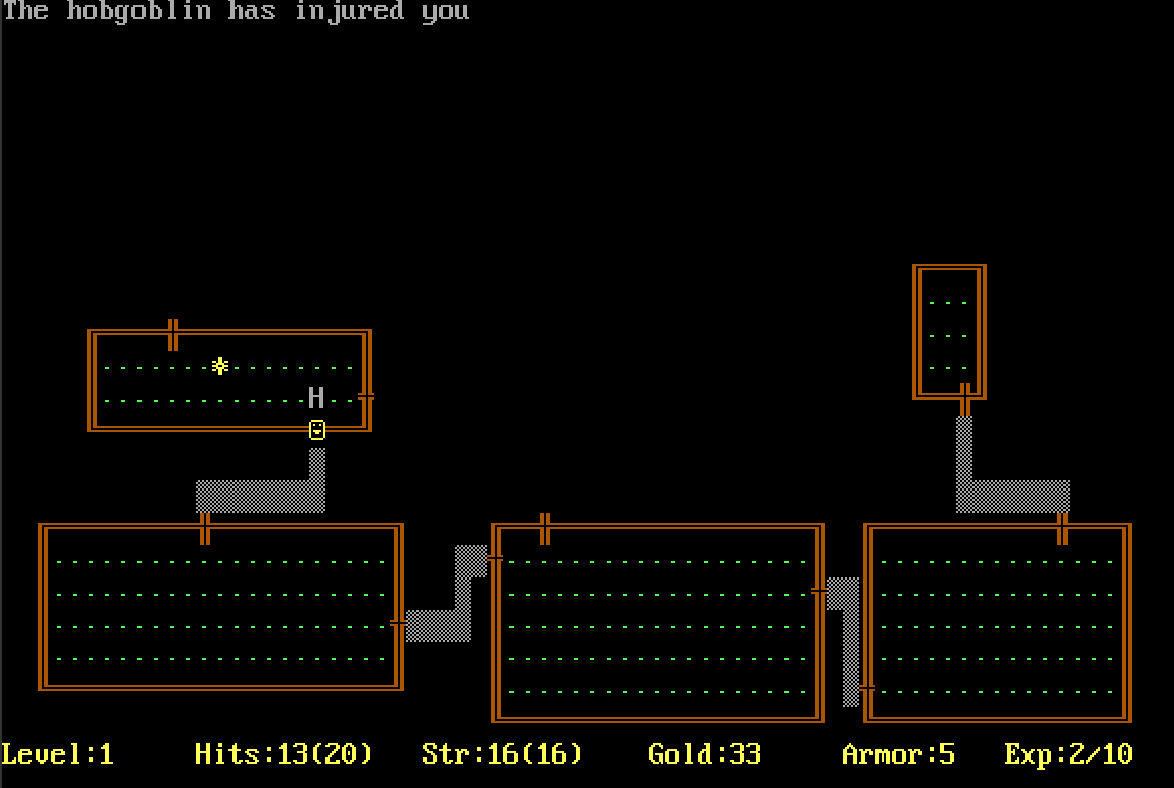
\includegraphics[width=12cm]{images/rogue/scr1.png}
	\caption{Widok główny gry Rogue}
	\label{Rogue:scr1}
\end{figure}
\FloatBarrier

Do sterowania w Rogue używana jest tylko klawiatura. Do poruszania przeznaczone są klawisze klawiatury numerycznej a do wykonywania akcji litery (na przykład klawisz 'I' służy do wyświetlenia ekwipunku). Aby zaatakować gracz musi poruszyć się w stronę przeciwnika będąc tuż przy nim. Wyświetlanie ekwipunku w grze Rogue pokazano na rysunku \ref{Rogue:scr2}. Manipulowanie przedmiotami w plecaku nie odbywa się w tym oknie, ale w głównym widoku gry za pomocą odpowiednich klawiszy odpowiadającym danemu przedmiotowi w ekwipunku. Przykładowo w celu wyrzucenia przedmiotu 'a +1, +1 mace` znajdującego się w ekwipunku na rysunku \ref{Rogue:scr2} trzeba wcisnąć klawisz 'd' odpowiadający za wyrzucanie przedmiotów i literę 'c' przypisaną obecnie do tego przedmiotu. 

\FloatBarrier
\begin{figure}[ht]
	\centering
	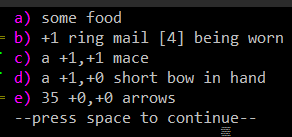
\includegraphics[width=10cm]{images/rogue/scr2.png}
	\caption{Ekran ekwipunku w Rogue}
	\label{Rogue:scr2}
\end{figure}
\FloatBarrier

Rogue zawiera proste proceduralnie generowane mapy, przykładowe dwie mapy pokazano na rysunku: \ref{Rogue:scr3}. Każda z map zawiera pokoje w układzie siatki 3x3, co szczególnie widać na mapie po prawej na rysunku \ref{Rogue:scr3}. Maksymalna liczba pokojów to dziewięć, ale może być ich mniej. Pokoje są połączone ze sobą korytarzami, a część przejść może być ukryta przed graczem, co wymusza częste korzystanie z komendy przeszukiwania dostępnej pod klawiszem 'S'. Pokoje i korytarze mogą zawierać ukryte pułapki, które można wykryć używając odpowiedniej komendy. Jedyną zmianą na głębszych poziomach są małe labirynty zastępujące wybrane pokoje.

\FloatBarrier
\begin{figure}[ht]
	\centering
	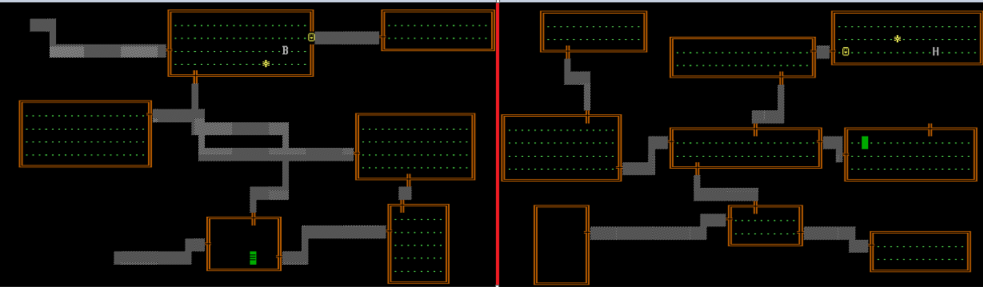
\includegraphics[width=16cm]{images/rogue/scr3.png}
	\caption{Przykładowe mapy w grze Rogue}
	\label{Rogue:scr3}
\end{figure}
\FloatBarrier

Z racji sporego wieku gry Rogue ciężko jest określić jej popularność, jednak z pewnością można stwierdzić, że jest to kluczowa dla gatunku roguelike gra, która stworzyła podwaliny jego głównych cech. Świadczy o tym między innymi sama nazwa gatunku roguelike, która oznacza "podobne do Rogue".



\subsection{Caves of Qud}
Caves of Qud to współczesny przykład rozwoju klasycznej formuły roguelike. Gra tworzona w silniku Unity przez studio Freehold Games wydana została w 2015 roku, lecz rozwijana jest do dzisiaj (stan na luty 2022). Gra posiada wszystkie cechy klasycznej gry roguelike: działa w systemie turowym, posiada permadeath oraz mapa gry oparta jest o siatkę kwadratów. Twórcy dodali wiele nowoczesnych rozwiązań i znacznie rozwinęli wiele mechanik gry. Caves of Qud osadzone jest w postapokaliptycznym świecie, w którym zaawansowana technologia miesza się z fantastycznymi rasami oraz magią.


Jednym z głównych wyróżników Caves of Qud na tle innych gier tego typu jest znacząco rozwinięty system proceduralnie generowanych map. Gra posiada otwarty świat o statycznie umiejscowionych obszarach, takich jak góry, pustynie oraz miasta. Na rysunku \ref{CoQ:scr1} przedstawiono przykładowe mapy wygenerowane w tej grze. Pomimo statycznego ustawienia konkretnych obszarów w grze, sam wygląd map jest proceduralnie generowany. Na wielu mapach mogą także zostać dodane obiekty takie jak ruiny lub obozowiska.

\FloatBarrier
\begin{figure}[ht]
	\centering
	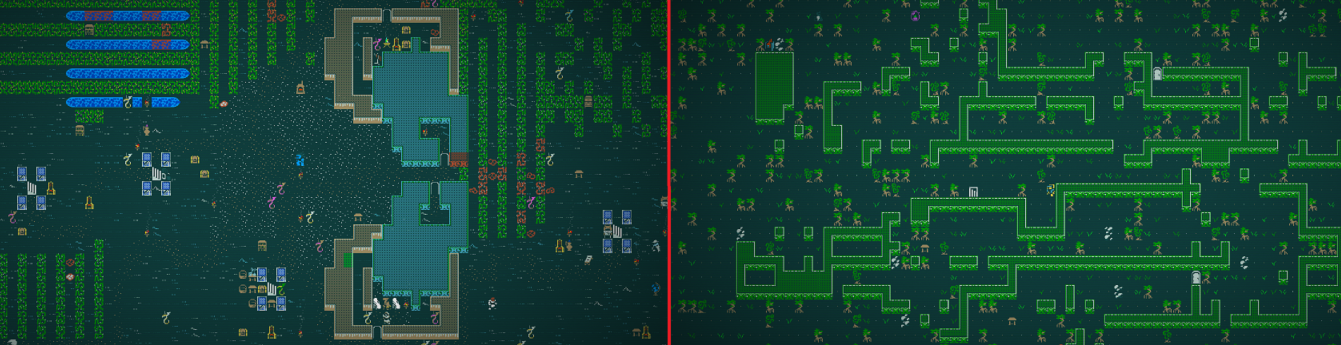
\includegraphics[width=16cm]{images/caves_of_qud/scr1.png}
	\caption{Przykładowe mapy w grze Caves of Qud. Po lewej wioska, po prawej dżungla z ruinami}
	\label{CoQ:scr1}
\end{figure}
\FloatBarrier

Główną i najbardziej interesującą metodą używaną w tej grze jest generowanie map oparte o Wave Function Collapse (Załamanie funkcji falowej) \cite{coq_wfc}. Metoda ta pozwala na generowanie wielu różnych typów map za pomocą jednego algorytmu. Działanie Wave Function Collapse wykorzystuje wzorzec, na podstawie którego tworzy większy wzór lokalnie podobny do oryginalnego, co przedstawiono na rysunku \ref{wfc} \cite{wfc_git}.

\FloatBarrier
\begin{figure}[ht]
	\centering
	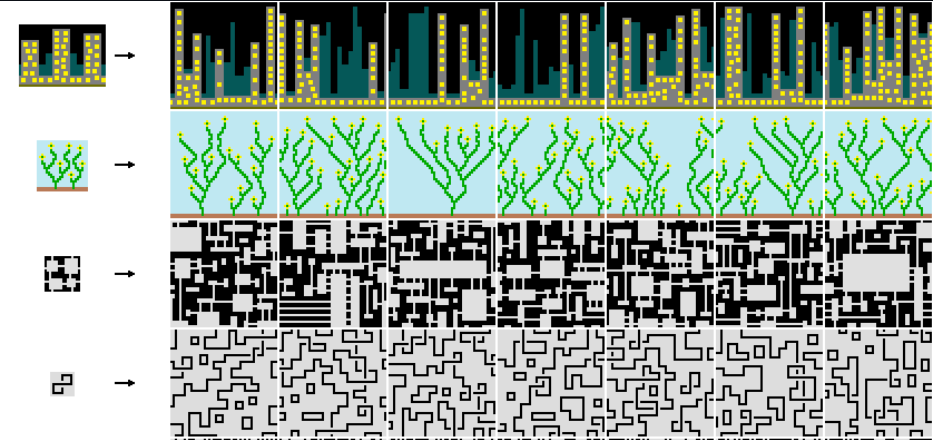
\includegraphics[width=12cm]{images/wfc.png}
	\caption{Przykład działania algorytmu opartego o Wave Function Collapse}
	\label{wfc}
\end{figure}
\FloatBarrier


Podobnie jak w grze Rogue, tutaj również do poruszania się używana jest klawiatura numeryczna oraz klawisze liter do wykonywania akcji. Caves of Qud umożliwia również granie wyłącznie za pomocą myszki. Gra oferuje bardziej przejrzystą grafikę typu \emph{pixel art} w formacie 16x24 piksele na jeden kwadrat na mapie, co przedstawiono na rysunku \ref{CoQ:scr3}. Mylącym może być, iż gra jest reprezentowana graficznie przez siatkę pionowych prostokątów, lecz w rzeczywistości traktuje je jako kwadraty -- ruch w każdym z ośmiu dostępnych kierunków zajmuje tyle samo czasu.

\FloatBarrier
\begin{figure}[ht]
	\centering
	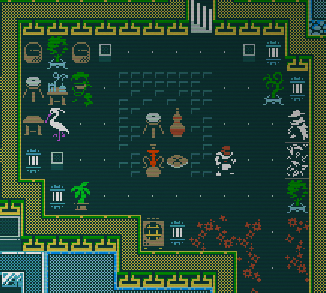
\includegraphics[width=65mm]{images/caves_of_qud/scr3.png}
	\caption{Zrzut ekranu z gry Caves of Qud}
	\label{CoQ:scr3}
\end{figure}
\FloatBarrier

Caves of Qud znacznie rozwinęło interfejs użytkownika, co znacząco wpływa na ułatwienie rozgrywki. Interfejs jest tu przejrzysty i prosty, dzięki czemu zmiana ekwipunku oraz używanie przedmiotów jest dużo łatwiejsze. Na rysunku \ref{CoQ:scr2} przedstawiono ekran ekwipunku.

\FloatBarrier
\begin{figure}[ht]
	\centering
	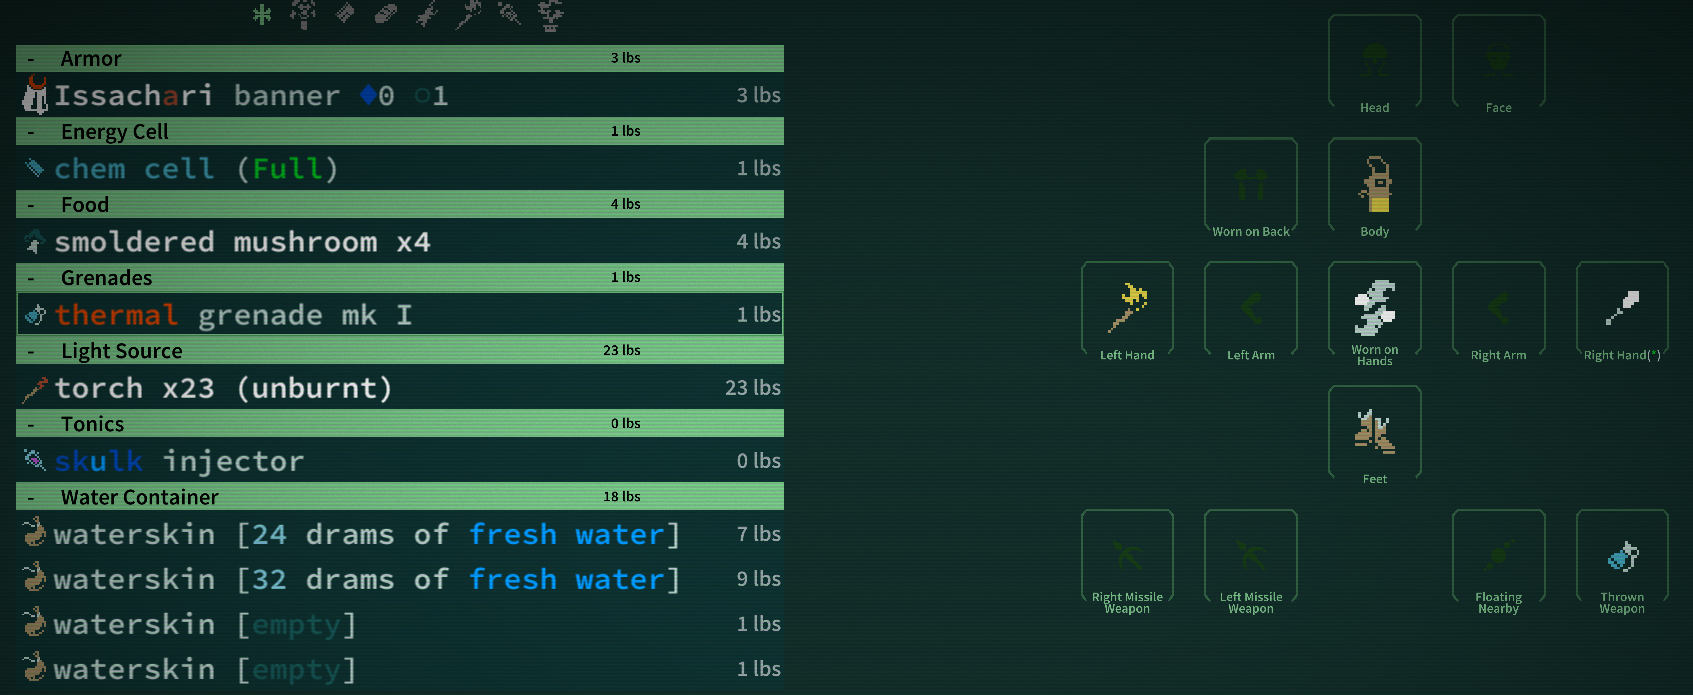
\includegraphics[width=14cm]{images/caves_of_qud/scr2.png}
	\caption{Ekran ekwipunku w Caves of Qud}
	\label{CoQ:scr2}
\end{figure}
\FloatBarrier

Interesującym rozwiązaniem w Caves of Qud jest system handlowy. W grze istnieje system głodu i pragnienia, gracz więc w celu uniknięcia śmierci musi nosić ze sobą zapasy wody oraz pożywienia. Zapasy te mają swoją wagę, więc można ich posiadać tylko ograniczoną liczbę. Walutą w tej grze jest woda pitna, która jest bardzo rzadko spotykana w postaci źródeł. Zdecydowana większość wody w zbiornikach naturalnych jest niezdatna do picia. Z tego powodu gracz zbiera wodę nie tylko dla zaspokojenia pragnienia, ale również w celu handlu ze spotykanymi handlarzami.

Gra Caves of Qud znacznie rozwija aspekt RPG -- odgrywania postaci. Dostępne są dwie rasy: mutant mający dostęp do fizycznych lub mentalnych mutacji oraz 'True Kin' będący niezmutowanym człowiekiem, który ma dostęp do cybernetycznych implantów. Poza typem wybiera się też pochodzenie postaci określające początkowy ekwipunek oraz bonusy do atrybutów. W trakcie gry gracz może dowolnie rozwijać swojego bohatera zwiększając wartości atrybutów takich jak siła, zręczność oraz inteligencja. Bohater uczy się też nowych umiejętności jak specjalizacja w posługiwaniu się konkretnym typem broni lub unikanie ataków.

W Caves of Qud proceduralne generowanie używane jest nie tylko do generowania map. W grze można znaleźć duże ilości proceduralnie tworzonych książek, z których część dotyczy także samej fabuły gry \cite{coq_history}. Oznacza to, że poza niektórymi, stałymi we wszystkich rozgrywkach, aspektami historii również część fabuły będzie inna w każdej nowej rozgrywce.

W odróżnieniu od większości gier tego typu, Caves of Qud posiada mocno rozwiniętą historię i rozbudowane główne zadania fabularne. Poza główną linią zadań gra oferuje też sporo losowych, które jednak są dosyć proste i najczęściej sprowadzają się do zdobycia konkretnego przedmiotu. Główne zadania są różnorodne, często polegają na odwiedzaniu fabularnych, rozbudowanych lokacji, obronie miasta przed atakiem lub nawet rozwiązywaniu zagadek.\\

Klasyczne gry typu roguelike posiadające zwykle dość wysoki poziom trudności rozgrywki wciąż uznawane są za dość niszowy gatunek. Poszczególne gry zyskują jednak relatywnie dużą popularność, czego przykładem jest gra Caves Qud, która w serwisie Steam posiada 4356 opinii z czego 95\% jest pozytywnych (stan na luty 2022) \cite{coq_steam}.



\subsection{The Binding of Isaac}

Gra The Binding of Isaac została stworzona w roku 2011 przez Edmunda McMillena i Floriana Himsla, a następnie w odświeżonej wersji jako The Binding of Isaac: Rebirth w roku 2014. W niniejszej pracy skupiono się na omówieniu The Binding of Isaac: Rebirth, gdyż jest to nowsza i bardziej popularna odsłona. Gra ta jest przykładem wzorowania się na gatunku roguelike, ale odejściu od części klasycznych założeń. Z gatunku zaczerpnięto losowo generowane mapy, losowe rozmieszczanie przedmiotów i przeciwników, oraz konieczność rozpoczęcia gry od początku w przypadku śmierci bohatera. Rozgrywka w The Binding Isaac dzieje się w czasie rzeczywistym, a ruch postaci nie jest ograniczony do siatki kwadratów. Z tego powodu gra jest bardziej dynamiczna, a walka zręcznościowa.

The Binding of Isaac odeszło od podziału mapy na kwadratową siatkę, ale wciąż korzysta z względnie prostej grafiki typu \emph{pixel art}, co przedstawiono na rysunku: \ref{tboi:scr1}.

\FloatBarrier
\begin{figure}[ht]
	\centering
	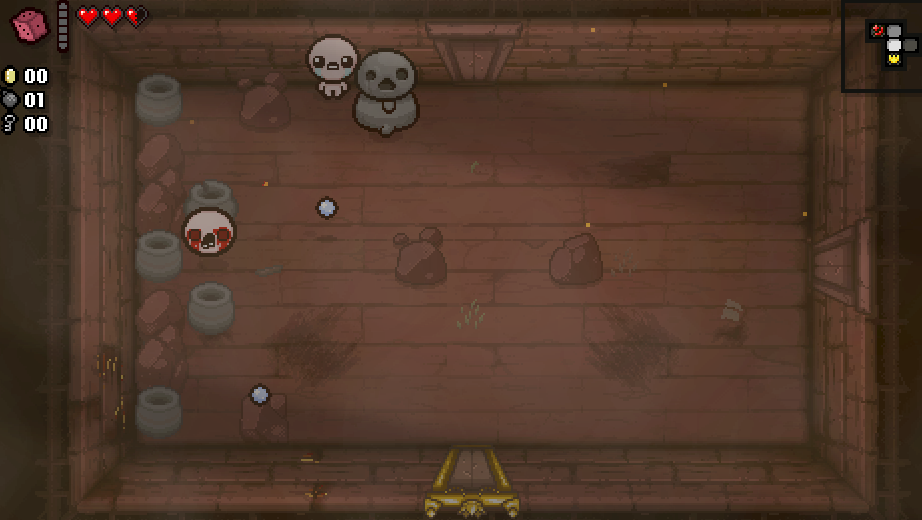
\includegraphics[width=10cm]{images/tboi/scr1.png}
	\caption{Przykład rozgrywki w The Binding of Isaac: Rebirth}
	\label{tboi:scr1}
\end{figure}
\FloatBarrier

Gracz wciela się początkowo w postać Isaaca, ale w trakcie rozgrywki może odblokować wiele nowych postaci, które różnią się początkowymi atrybutami -- zdrowie, prędkość i siła ataku oraz posiadanymi przedmiotami. Gra nie posiada typowego ekwipunku takiego jak zbroja i broń, zamiast tego w grze zbiera się nieograniczoną liczbę przedmiotów, które zapewniają pasywne bonusy. Bonusy te wzmacniają postać na wiele różnych sposobów, od podstawowych zwiększających zdrowie lub atak po takie, które zmieniają pociski wstrzeliwane przez gracza na zupełnie inną postać. Jednym z głównym atutów The Binding of Isaac są możliwe kombinacje przedmiotów. Przykładowo jeśli gracz zdobędzie przedmiot, dzięki któremu pociski postaci będą się same kierowały na przeciwników, a następnie przedmiot, który zamienia pociski na promień lasera, to ten promień będzie zaginany tak, aby zawsze trafiać przeciwników bez konieczności celowania, co pokazano na rysunku \ref{tboi:scr2}.


\FloatBarrier
\begin{figure}[ht]
	\centering
	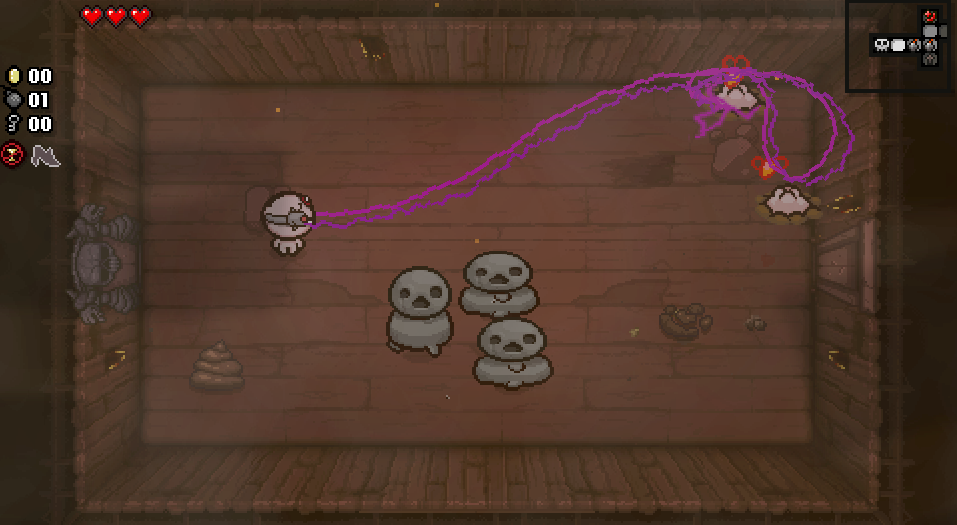
\includegraphics[width=10cm]{images/tboi/scr2.png}
	\caption{Przykład kombinacji przedmiotów w The Binding of Isaac: Rebirth}
	\label{tboi:scr2}
\end{figure}
\FloatBarrier

W grze The Binding of Isaac za sterowanie postacią odpowiadają klawisze 'W', 'A', 'S', 'D' , a za strzelanie klawisze strzałek, do używania przedmiotów jest też używana spacja i klawisz 'Q'. Proste sterowanie jest kolejnym powodem przystępności tej gry.

 W porównaniu do innych gier roguelike losowo generowane mapy w The Binding of Isaac są znacznie prostsze. Gra składa się z wielu poziomów podzielonych na pokoje, każdy z poziomów zakończony jest walką z silnym przeciwnikiem. Pokoje są wybierane losowo z puli przygotowanej przez twórców, a ich rozkład i połączenia są losowo generowane. Na rysunku \ref{tboi:scr3} przedstawiono przykładowy układ poziomów. Z każdym kolejnym poziomem liczba pokojów jest coraz większa, ale jakość napotykanych przedmiotów nie wzrasta. Przedmioty są kompletnie losowe, dlatego czasem już nawet po pierwszym poziomie postać gracza może posiadać kilka najsilniejszych przedmiotów. 

\FloatBarrier
\begin{figure}[ht]
	\centering
	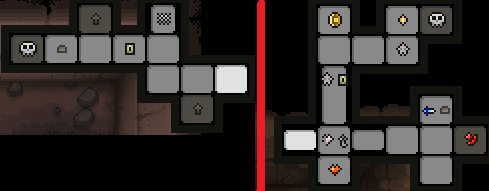
\includegraphics[width=12cm]{images/tboi/scr3.png}
	\caption{Przykładowe układy poziomów w The Binding of Isaac: Rebirth}
	\label{tboi:scr3}
\end{figure}
\FloatBarrier


Jedną z cech gier gatunku roguelike, które implementuje The Binding of Isaac jest permadeath. W porównaniu do innych tytułów, na których ukończenie trzeba często poświęcić parę godzin, ukończenie The Binding of Isaac sprawnemu graczowi zajmie około godzinę. W wyniku tego rozpoczynanie rozgrywki od początku nie jest tak dotkliwe i zachęca do częstego, powtórnego przechodzenia gry.


The Binding of Isaac: Rebirth jest jedną z najbardziej popularnych gier z gatunku roguelike. Na serwisie Steam posiada 166244 opinii, w tym 97\% pozytywnych (stan na luty 2022) \cite{tboi_steam}. Dowodzi to, że przeciętny gracz woli dynamiczną, rozgrywaną w czasie rzeczywistym rozgrywkę, od wolnej i taktycznej rozgrywki turowej. Kolejnym dowodem popularności tej gry jest wydana w 2018 roku gra planszowa The Binding of Isaac: Four Souls, która w tydzień zebrała ponad milion dolarów na serwisie Kickstarter \cite{tboi_4souls}.



\clearpage	

\section{Szczegółowy opis gry}

W tym rozdziale przedstawiono wszystkie elementy i możliwości gry stworzonej na potrzeby niniejszej pracy.


\subsection{Główne założenia}
Zrealizowana na potrzeby niniejszej pracy gra spełnia podstawowe cechy klasycznych rozgrywek z gatunku roguelike:

\begin{itemize}
	\item oparta jest o system turowy,
	\item zawiera plansze generowane proceduralnie,
	\item rozmieszczenie przeciwników i przedmiotów jest losowe,
	\item mapy są w postaci siatki kwadratów, ruch gracza ograniczony jest do poruszania się po nich,
	\item bohater posiada ekwipunek, który może założyć -- zbroje i broń,
	\item gra posiada przedmioty, których można użyć -- mikstury i magiczne zwoje,
	\item permadeath - śmierć kończy rozgrywkę, brak możliwości zapisu i wczytania stanu rozgrywki.		
\end{itemize}

Projekt gry posiada też kilka bardziej nowoczesnych aspektów:
\begin{itemize}
	\item grafika typu \emph{pixel art},
	\item rozwinięty, prostszy w użytkowaniu interfejs,			
	\item system prezentowania z krokami proceduralnego generowania map.
\end{itemize}

Gra składa się z sześciu różnorodnych, proceduralnie generowanych poziomów. Gracz napotyka coraz trudniejszych przeciwników w kolejnych poziomach, a także znajduje coraz lepszy ekwipunek i przedmioty. Celem gry jest pokonanie ostatniego przeciwnika -- potężnego szlamu, znajdującego się na ostatnim poziomie. Aby ukończyć grę gracz powinien eksplorować kolejne poziomy w celu odnalezienia silniejszych przedmiotów i ekwipunku  niezbędnych przy walce z trudniejszymi przeciwnikami.  Gra osadzona jest w fantastycznym, średniowiecznym świecie, w którym spotkać można rycerzy, gobliny i orków, a także magiczne mikstury i zwoje.


\subsection{Opis menu głównego gry}
Po uruchomieniu gry pierwsze, co zobaczy gracz to główne menu przedstawione na rysunku \ref{mygame:scr1}. Menu składa się z żółtego tytułu gry, oraz czterech opcji. Poruszać się po menu można za pomocą klawiszy strzałek, aktualnie wybrana opcja jest zaznaczona na zielono, a wybór opcji przeprowadzany jest klawiszem enter.

\FloatBarrier
\begin{figure}[ht]
	\centering
	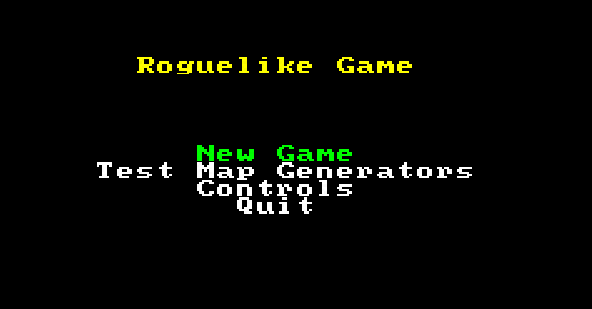
\includegraphics[width=10cm]{images/mygame/scr1.png}
	\caption{Menu główne gry}
	\label{mygame:scr1}
\end{figure}
\FloatBarrier

Menu składa się z następujących opcji:
\begin{itemize}
	\item 'New Game' -- rozpoczęcie nowej gry,
	\item 'Test Map Generators' -- otwiera menu testera proceduralnego generowania map,			
	\item 'Controls' -- otwiera listę komend dostępnych w grze,
	\item 'Quit' -- zamknięcie programu.
\end{itemize}


\subsection{Sterowanie w grze}
 Główną metodą poruszania się postaci jest klawiatura numeryczna, co używane jest od dawna w gatunku roguelike. Jest to także najwygodniejsza kombinacja klawiszy przy możliwości ruchu w ośmiu kierunkach -- dół, góra, prawo, lewo oraz skosy, schemat poruszania się przy użyciu klawiatury numerycznej przedstawiono na rysunku \ref{numpad_controls}. Nie wszystkie klawiatury, a szczególnie te w laptopach, posiadają klawiaturę numeryczną, dlatego gra posiada też alternatywne sterowanie oparte o klawisze strzałek i klawisze liter. Klawisz '5' w przypadku klawiatury numerycznej używany jest do pomijania tury, co jest istotną możliwością w grze turowej. Jednokrotne naciśnięcie klawisza odpowiadającego za ruch porusza postać gracza o jedno pole w danym kierunku, jeżeli nie jest ono zajmowane przez ścianę. Jeśli pole na które porusza się gracz zajmowane jest przez przeciwnika, to zamiast ruchu postać gracza wykona atak przeciwko temu przeciwnikowi, jest to standardowa metoda ataku w tego typu grach.
 
\FloatBarrier
\begin{figure}[ht]
	\centering
	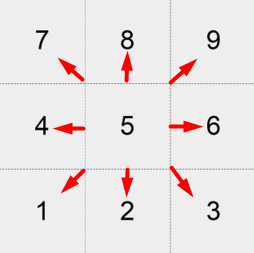
\includegraphics[width=4cm]{images/custom/numpad_controls.png}
	\caption{Schemat sterowania na klawiaturze numerycznej}
	\label{numpad_controls}
\end{figure}
\FloatBarrier

Objaśnienia sterowania i lista dostępnych akcji w grze z menu głównego za pomocą opcji 'Controls' na rysunku \ref{mygame:scr2} przedstawiono widok dostępny po wybraniu tej opcji.

\FloatBarrier
\begin{figure}[ht]
	\centering
	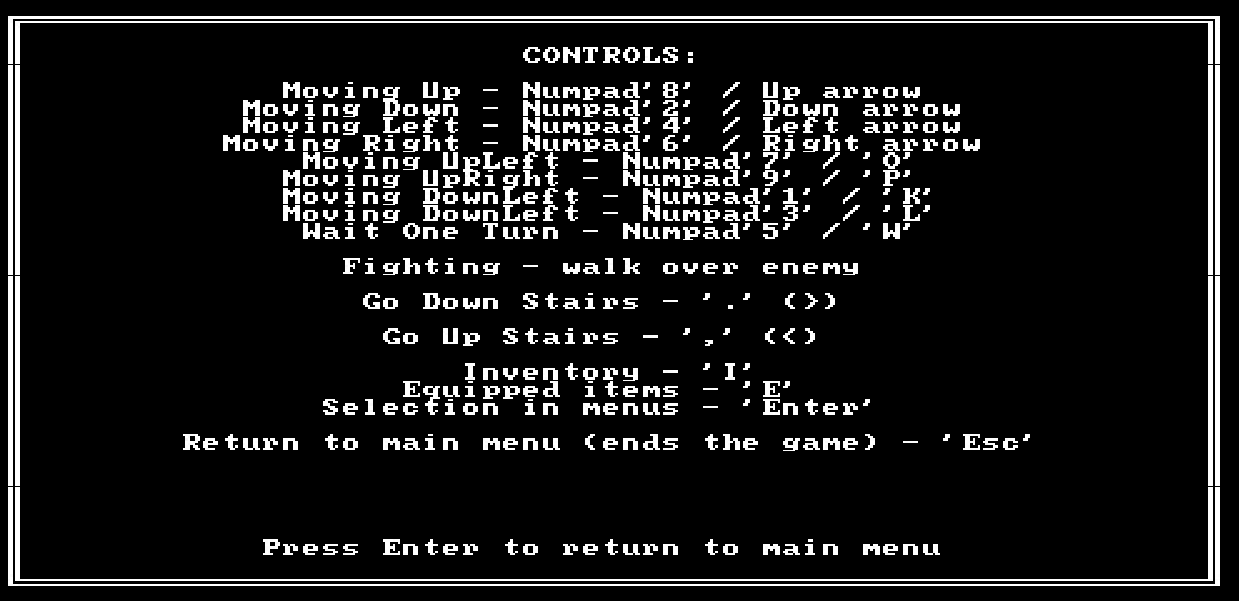
\includegraphics[width=16cm]{images/mygame/scr2.png}
	\caption{Objaśnienia sterowania w grze}
	\label{mygame:scr2}
\end{figure}
\FloatBarrier



Poniżej wyjaśnienie wszystkich komend dostępnych w grze w kolejności z rysunku \ref{mygame:scr2}, Oznaczenie NumpadX oznacza klawisz cyfry X z klawiatury numerycznej. Oznaczenie 'X' oznacza klawisz litery lub znaku X:

\begin{enumerate}
	\item Numpad8 / klawisz strzałki w górę -- poruszenie się w górę,
	\item Numpad2 / klawisz strzałki w dół -- poruszenie się w dół,
	\item Numpad4 / klawisz strzałki w lewo -- poruszenie się w lewo,
	\item Numpad6 / klawisz strzałki w prawo -- poruszenie się w prawo,
	\item Numpad7 / 'O' -- poruszenie się na ukos -- góra, lewo,
	\item Numpad9 / 'P' -- poruszenie się na ukos -- góra, prawo,
	\item Numpad1 / 'K' -- poruszenie się na ukos -- dół, lewo,
	\item Numpad3 / 'L' -- poruszenie się na ukos -- dół, prawo,
	\item Numpad5 / 'W' -- pominięcie jednej tury,
	\item ',' (klawisz przecinka) -- zejście w dół po schodach,
	\item '.' (klawisz kropki) -- wejście w górę po schodach,
	\item 'G' -- podniesienie przedmiotu,
	\item 'I' -- otwarcie menu ekwipunku,
	\item 'E' -- pokazuje obecnie wyekwipowane przedmioty,
	\item klawisz Enter -- wybór opcji w menu,
	\item klawisz Esc -- powrót do menu głównego, kończy to obecną rozgrywkę,
	\item klawiszem Enter powrócić można z menu `Controls` do menu głównego.
\end{enumerate}


\subsection{Okno gry}
Po rozpoczęciu nowej gry gracz zobaczy okno z wycinkiem mapy wycentrowanym na postać gracza, a także okno dziennika zdarzeń i pasek punktów życia, co pokazano na rysunku \ref{mygame:game_window}. Widok mapy jest powiększonym wycinkiem poziomu, przesuwającym się razem z graczem. Na mapie poza ścianami zaznaczone są też pola podłogi za pomocą białej kropki. Jest to przydatne do przeliczania odległości w grach opierających się o ruch na siatce kwadratów. W dzienniku zdarzeń zapisywane są wydarzenia z gry takie jak podnoszenie przedmiotu i ataki gracza lub przeciwników. Pasek życia posiada liczbową prezentację punktów życia w postaci [aktualne punkty zdrowia / maksymalne punkty zdrowia], oraz graficzną reprezentację -- czerwony pasek zmniejszający się wraz ze spadkiem zdrowia. Gracz posiada pole widzenia o określonym zasięgu, które działa w sposób realistyczny to znaczy będąc blisko wejścia do pokoju jest on w stanie zobaczyć tylko jego skrawek, a nie cały pokój, co widać na rysunku \ref{mygame:game_window}. Szarym kolorem zaznaczone są zapamiętane, odwiedzone wcześniej obszary, które aktualnie nie znajdują się w bezpośrednim polu widzenia bohatera. Na obszarach, które gracz pamięta, ale nie widzi ich obecnie zaobserwować można tylko układ podłóg i ścian.Przeciwników i przedmioty zauważyć można tylko w bezpośrednim polu widzenia.

\FloatBarrier
\begin{figure}[ht]
	\centering
	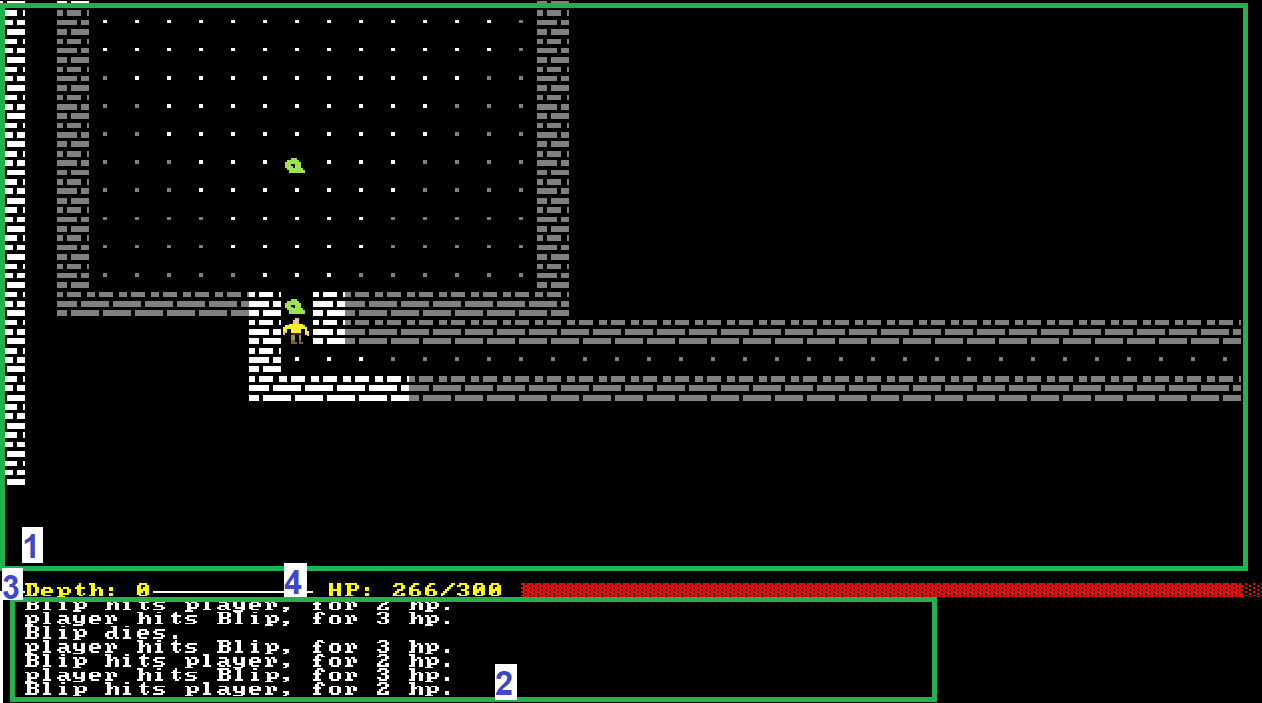
\includegraphics[width=16cm]{images/mygame/game_window.png}
	\caption{Widok główny gry. 1 - aktualny wycinek mapy, 2 - dziennik zdarzeń, 3 - aktualny poziom, 4 - pasek zdrowia. Żółta postać to gracz, a zielone postacie to gobliny -- jeden z typów przeciwników }
	\label{mygame:game_window}
\end{figure}
\FloatBarrier


\subsection{Opis poziomów}
Gra składa się z sześciu poziomów oferujących różnorodnych przeciwników i przedmioty. W tej sekcji w celu prezentacji wyglądu poszczególnych poziomów posłużono się testerem proceduralnie generowanych map. Poziomy zaprezentowano w kolejności w jakiej występują w trakcie rozgrywki. Mapy na poziomach 1-5 są proceduralnie generowane, więc przy każdej nowej rozgrywce ich wygląd będzie podobny, ale odmienny. Również rozmieszczenie przeciwników i przedmiotów na poziomach jest za każdym razem losowe. Akcja gry ma miejsce w podziemnych lochach połączonych z jaskiniami, kolejne poziomy są umieszczone coraz głębiej, dlatego są połączone ze sobą schodami, których położenie również jest losowe. Gracz ma możliwość swobodnego wracania do poprzednich poziomów.

\subsubsection{Poziom 1}
Poziom pierwszy to kilka prostych pokojów połączonych ze sobą korytarzami, przykładowy układ mapy przedstawiono na rysunku \ref{mygame:map1}. Na poziomie tym napotkać można najprostszych przeciwników: goblin oraz mały szlam. Istnieje też mała szansa, że w pokoju z goblinami pojawi się też trudniejszy przeciwnik -- ork. Na poziomie tym znaleźć można podstawowy pancerz i miecz, a także mikstury uzdrawiające i zwoje uśpienia, które są szczególnie przydatne w walkach z trudniejszymi przeciwnikami w dalszych poziomach.

\FloatBarrier
\begin{figure}[ht]
	\centering
	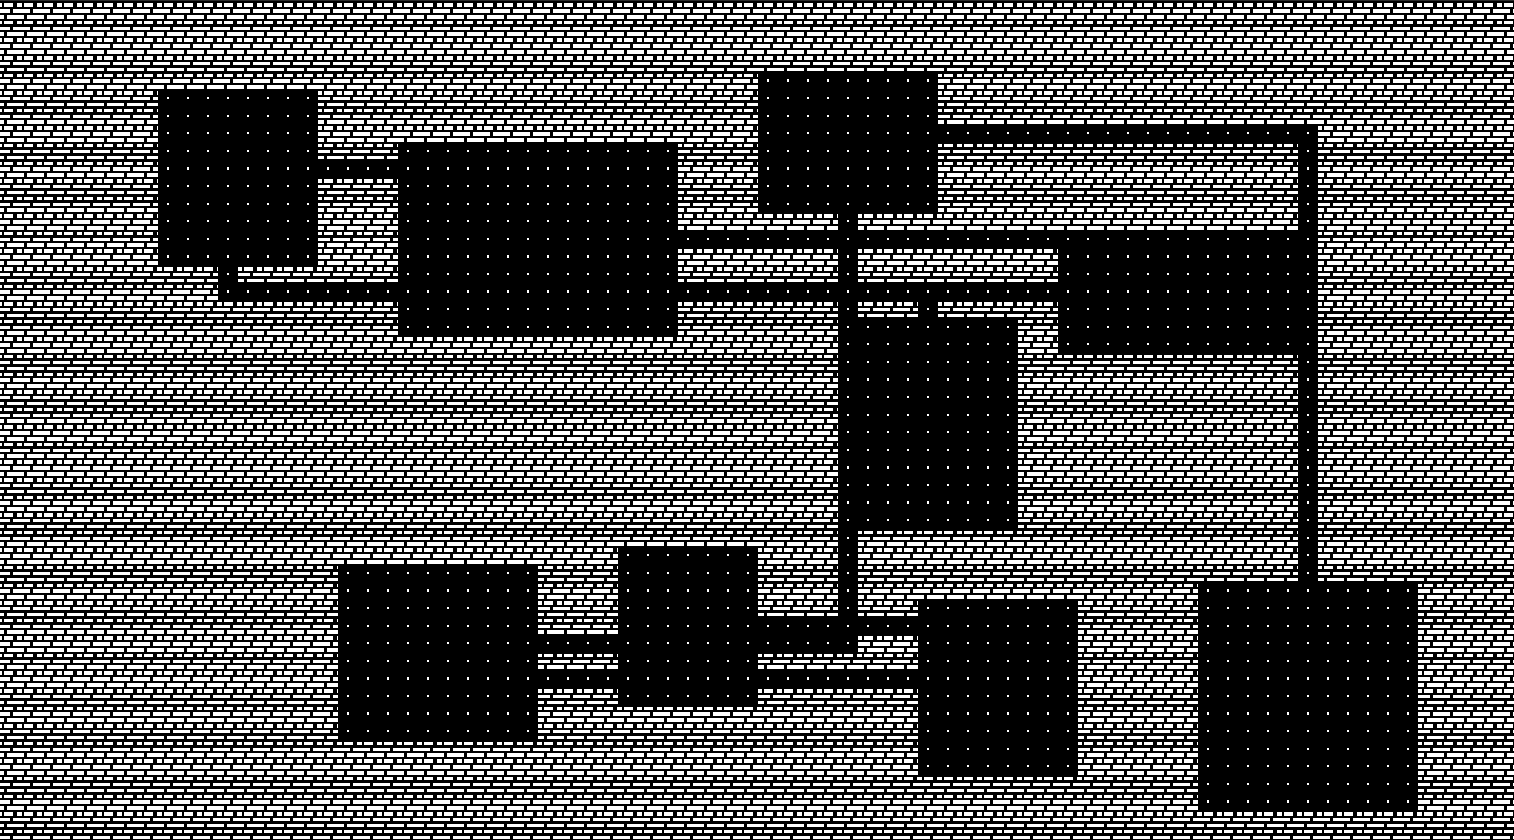
\includegraphics[width=12cm]{images/mygame/map1.png}
	\caption{Przykładowy układ poziomu pierwszego}
	\label{mygame:map1}
\end{figure}
\FloatBarrier


\subsubsection{Poziom 2}
Poziom drugi to bardziej rozwinięta wersja poziomu pierwszego z większą liczbą pokojów i inną metodą generacji. Przykładowy poziom drugi przedstawiono na rysunku \ref{mygame:map2}.Można na nim spotkać gobliny z poprzedniego poziomu a także trudniejszych: orków i rycerza. Szczególnie trudnym przeciwnikiem na tym poziomie jest rycerz, który wyposażony został w mocną zbroję i miecz. Przedmioty te można zdobyć  po jego pokonaniu. W pokoju z rycerzem jest też szansa na znalezienie potężniejszych magicznych zwojów - kuli ognia, oraz  teleportacji. Na poziomie tym można też znaleźć małe ilości mocniejszych mikstur uzdrowienia, oraz zwoje magicznych pocisków.


\FloatBarrier
\begin{figure}[ht]
	\centering
	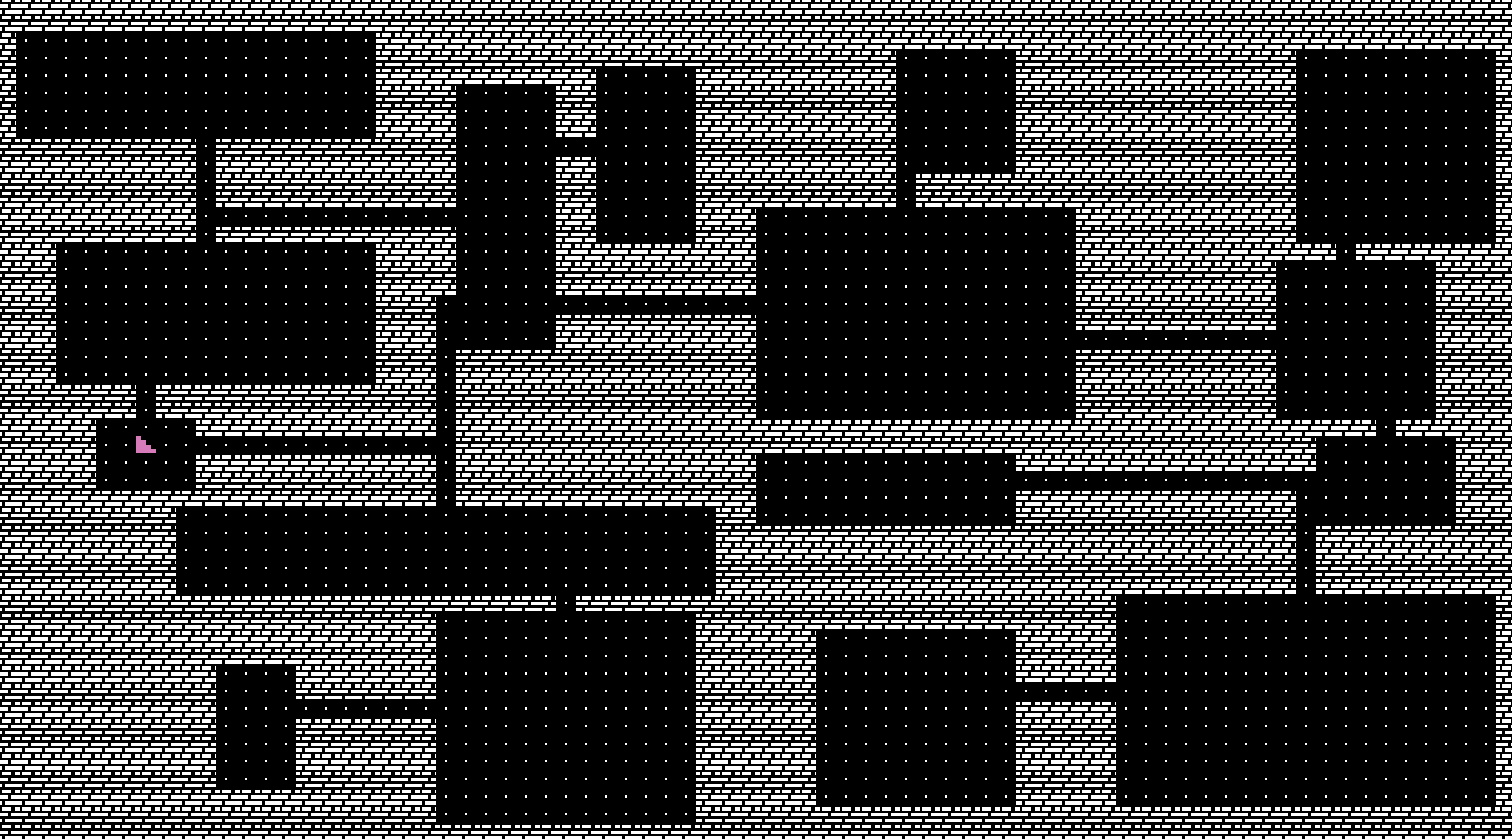
\includegraphics[width=14cm]{images/mygame/map2.png}
	\caption{Przykładowy układ poziomu drugiego}
	\label{mygame:map2}
\end{figure}
\FloatBarrier


\subsubsection{Poziom 3}
Poziom trzeci to duża jaskinia wypełniona masą goblinów i orków. Przykładowy widok poziomu trzeciego przedstawiono na rysunku \ref{mygame:map3}. Mimo, że nie spotyka się tu trudniejszych przeciwników niż orkowie, to trudnością tego etapu jest duża ich liczba, oraz otwarty teren. Taki układ mapy, w przeciwieństwie do ciasnych korytarzy poprzednich poziomów, może łatwo doprowadzić do otoczenia gracza przez wielu przeciwników.

\FloatBarrier
\begin{figure}[ht]
	\centering
	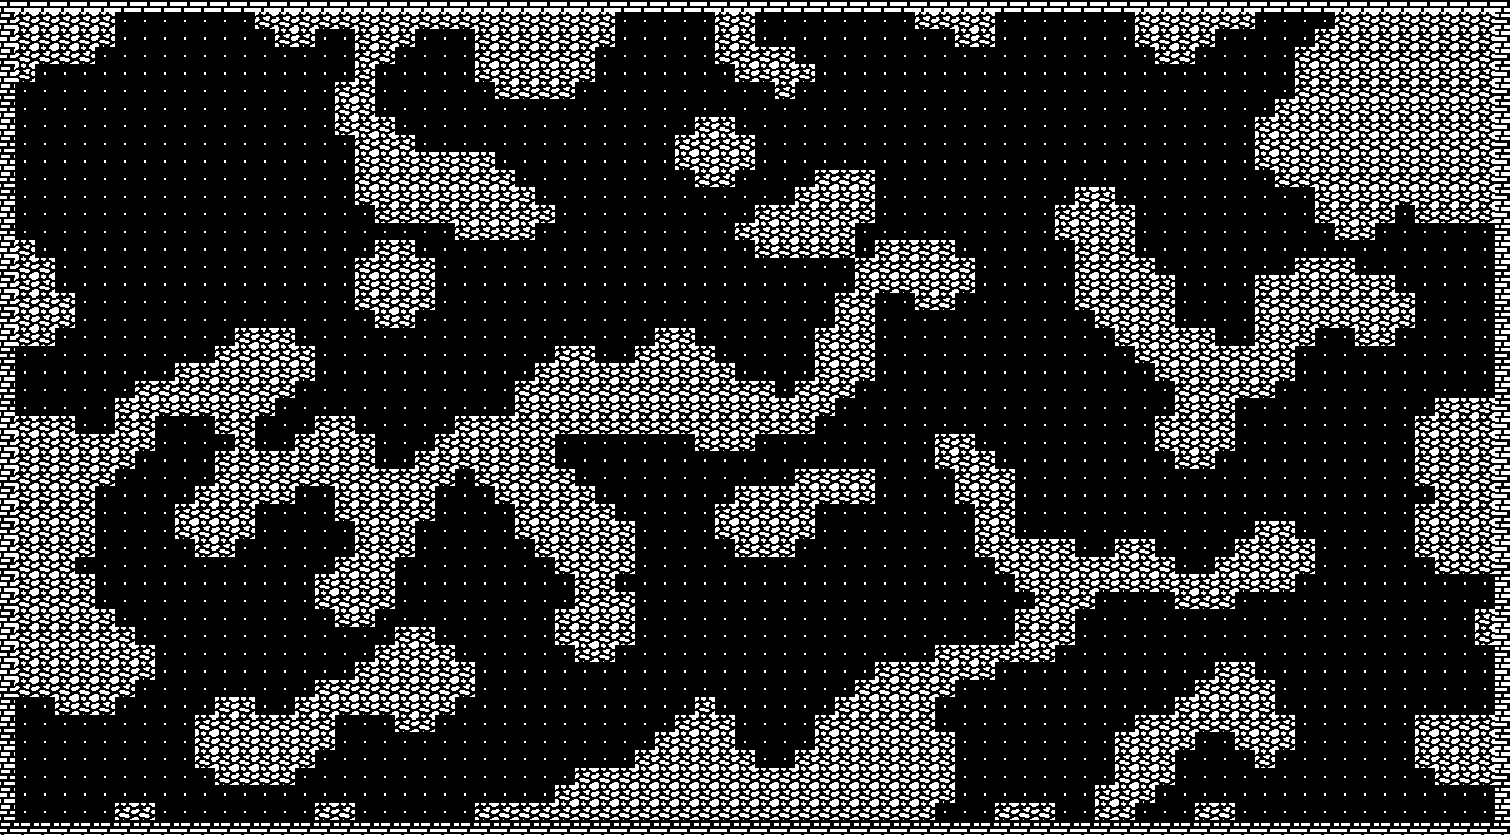
\includegraphics[width=12cm]{images/mygame/map3.png}
	\caption{Przykładowy układ poziomu trzeciego}
	\label{mygame:map3}
\end{figure}
\FloatBarrier


\subsubsection{Poziom 4}
Poziom czwarty to kolejna jaskinia, tym razem z dużo większym obszarem w centrum, oraz okazjonalnymi ciasnymi odnogami. Przykładowy widok poziomu czwartego przedstawiono na rysunku \ref{mygame:map4}. Na poziomie tym można spotkać dużą liczbę prostych małych szlamów z pierwszego poziomu, a także sporo ich większych odmian. Większy szlam poza byciem silniejszą odmianą posiada też specjalną zdolność -- po śmierci rozpadnie się na kilka małych szlamów. Na tym poziomie można też znaleźć mocniejszą zbroję i miecz, a także duże mikstury uzdrowienia i zwoje obszarowego uśpienia.

\FloatBarrier
\begin{figure}[ht]
	\centering
	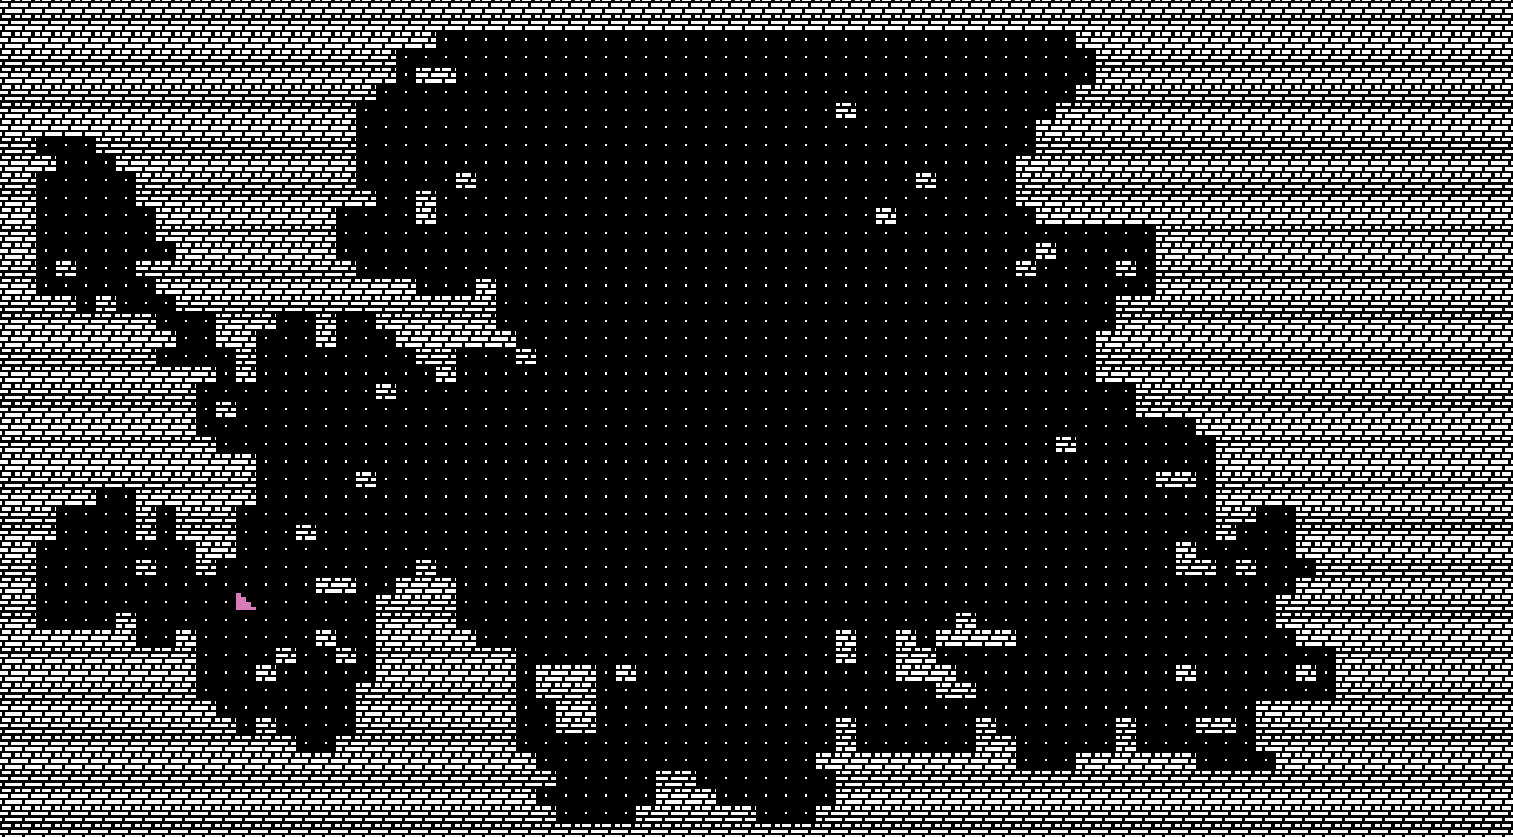
\includegraphics[width=12cm]{images/mygame/map4.png}
	\caption{Przykładowy układ poziomu czwartego}
	\label{mygame:map4}
\end{figure}
\FloatBarrier

\subsubsection{Poziom 5}
Poziom piąty to duży obszar podzielony na pokoje bezpośrednio połączone ze sobą, bez korytarzy. Przykładową mapę poziomu piątego przedstawiono na rysunku \ref{mygame:map5}. Na tym poziomie spotkać można najmocniejszych przeciwników: rycerzy oraz łotrzyków. W trakcie eksploracji poziomu piątego odnaleźć można najmocniejszą w grze zbroję oraz miecz, co będzie dla gracza szczególnie przydatne na poziomie szóstym.

\FloatBarrier
\begin{figure}[ht]
	\centering
	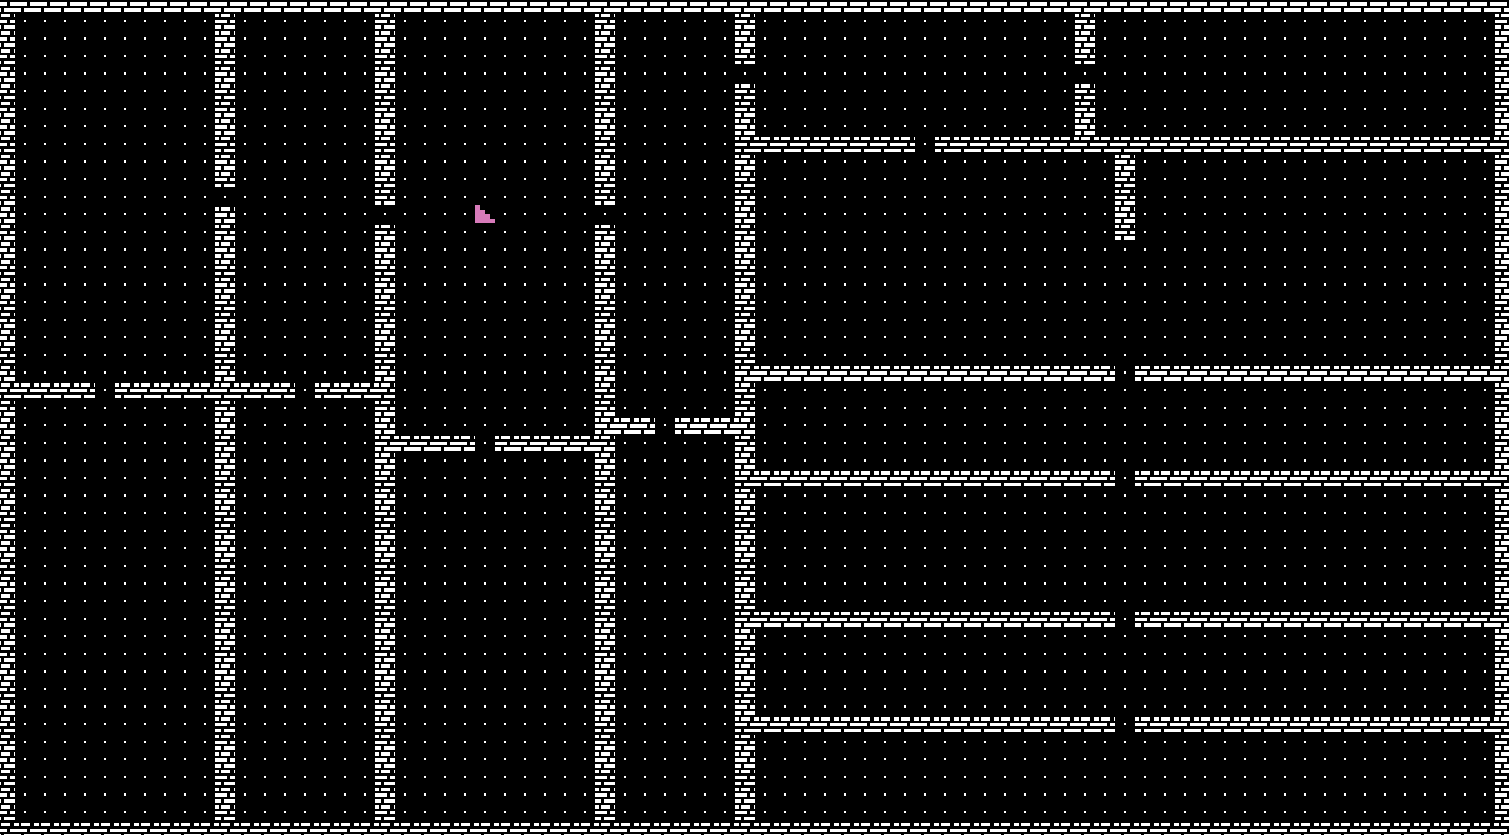
\includegraphics[width=12cm]{images/mygame/map5.png}
	\caption{Przykładowy układ poziomu piątego}
	\label{mygame:map5}
\end{figure}
\FloatBarrier


\subsubsection{Poziom 6}
Ostatni poziom jest wielką, otwartą przestrzenią. Na tym poziomie gracz znajduje się tylko jeden przeciwnik -- potężny szlam, którego pokonanie jest celem gry. Potężny szlam jest silniejszą wariacją szlamów, na które rozpada się po śmierci, one z kolei po śmierci rozpadną się na małe szlamy. Aby ukończyć grę należy go pokonać oraz zejść schodami w dół.


\subsection{Przedmioty oraz ich używanie}
W grze gracz przez eksplorację znaleźć może wiele różnorodnych przedmiotów, których używanie jest konieczne w celu ukończenia gry. Przedmioty dzielą się na zbroje, broń, mikstury oraz magiczne zwoje. Aby podnieść przedmiot gracz musi przejść na zajmowane przez przedmiot pole a następnie wcisnąć klawisz 'G'. Na rysunku \ref{mygame:item_room} przedstawiono pokój wypełniony przedmiotami.

\FloatBarrier
\begin{figure}[ht]
	\centering
	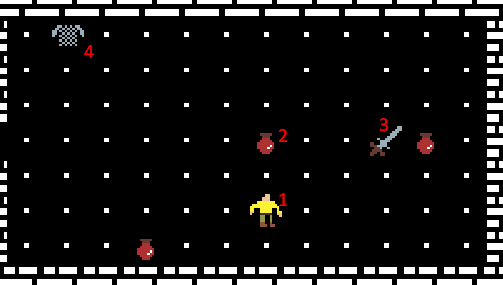
\includegraphics[width=9cm]{images/mygame/item_room.png}
	\caption{Pokój z przedmiotami. 1 - postać gracza, 2 - mikstura zdrowia, 3 - broń, 4 - zbroja }
	\label{mygame:item_room}
\end{figure}
\FloatBarrier


\subsubsection{Okna ekwipunku}
Gracz w każdej chwili może sprawdzić swój ekwipunek klawiszem 'I' -- ekran zaprezentowano na rysunku \ref{mygame:inv}. Wyboru przedmiotu dokonuje się za pomocą strzałek i klawisza Enter -- litera po lewej stronie przy aktualnie wybranym przedmiocie jest zaznaczona na zielono. Innym sposobem wybrania przedmiotu jest wciśnięcie przypisanej mu po lewej stronie litery w nawiasach. Dopisek '<EQUIPPED>' po prawej stronie danego przedmiotu oznacza, że jest on aktualnie założony przez postać gracza. Zielone liczby oznaczają zasoby danego przedmiotu. Na rysunku \ref{mygame:inv}  zaobserwować można, że gracz posiada cztery mikstury uzdrawiające 'Health potion'. Klawiszem Esc można wyjść z menu ekwipunku i powrócić do gry.

\FloatBarrier
\begin{figure}[ht]
	\centering
	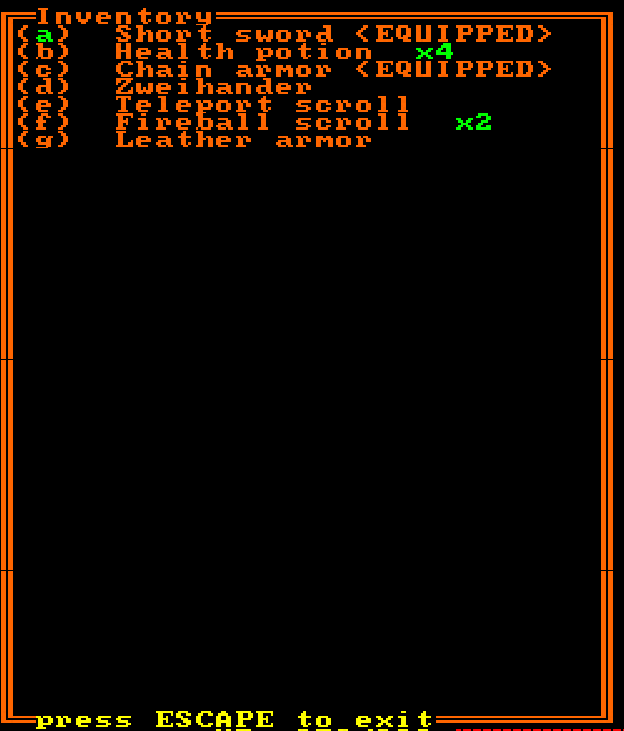
\includegraphics[width=8cm]{images/mygame/inv.png}
	\caption{Okno ekwipunku}
	\label{mygame:inv}
\end{figure}
\FloatBarrier

Po wybraniu przedmiotu wyświetla się menu wyboru akcji dostępnych dla każdego przedmiotu. Przykładowe dostępne akcje dla mikstury uzdrawiającej przedstawiono na rysunku \ref{mygame:item_menu}. Każdy przedmiot można wyrzucić za pomocą akcji 'drop' -- spowoduje to wyrzucenie przedmiotu na pole zajmowane przez gracza. W przypadku niezałożonych zbroi i broni dostępna jest opcja 'Equip' powodująca wyekwipowanie danego przedmiotu. Konsekwentnie, założone przedmioty posiadają akcję 'UnEquip', która pozwala na ściągnięcie danego przedmiotu. Mikstury i zwoje posiadają akcję 'Use' pozwalająca na użycie danego przedmiotu. Niektóre przedmioty są używane od razu na postaci gracza, a inne pozwalają na wybranie celu.

\FloatBarrier
\begin{figure}[ht]
	\centering
	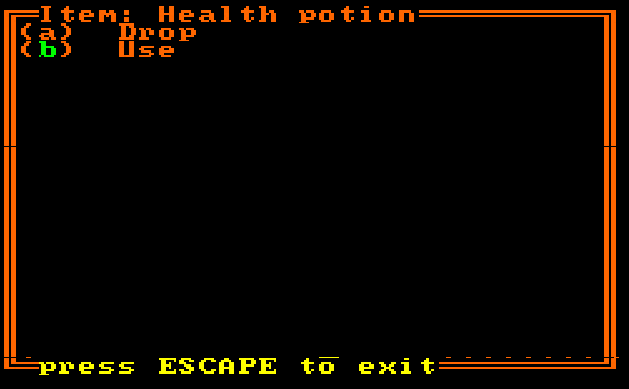
\includegraphics[width=75mm]{images/mygame/item_menu.png}
	\caption{Okno akcji przedmiotu z ekwipunku}
	\label{mygame:item_menu}
\end{figure}
\FloatBarrier

\subsubsection{Zbroje i broń}
Każda postać w grze posiada poziom obrony, który obniża wartość otrzymywanych obrażeń. Poziom ten zwiększyć można za pomocą zbroi zakładanych na poszczególne części ciała: głowę, tors, ręce oraz nogi. W grze w kolejnych poziomach spotkać można coraz lepsze rodzaje zbroi, dzięki czemu postać gracza jest coraz wytrzymalsza.

Postać gracza oraz przeciwnicy posiadają również wartość ataku, która określa liczbę zadawanych w trakcie akcji obrażeń. Wartość tę można zwiększyć zbierając broń rozsianą po poziomach. Lepsze rodzaje broni znaleźć można w późniejszych poziomach, dzięki czemu gracz, który dokładnie eksploruje plansze będzie zadawał coraz więcej obrażeń. Reprezentację graficzną zbroi oraz broni zaobserwować można na rysunku \ref{mygame:item_room}.


\subsubsection{Mikstury}
Postać gracza posiada określoną liczbę punktów zdrowia 'HP', które zmniejszają się wskutek ataków przeciwników. Aby zregenerować zdrowie gracz musi znaleźć mikstury uzdrawiające. W grze dostępne są dwie wersje tych mikstur -- zwykła 'Health potion' oraz większa 'Great health potion', która leczy więcej punktów zdrowia. Użycie mikstur jest natychmiastowe, a celem zawsze jest postać gracza. Wygląd mikstur został pokazany na rysunku \ref{mygame:item_room}.


\subsubsection{Zwoje}
Kolejnym typem przedmiotów są magiczne zwoje. Zwoje zapewniają wiele różnorodnych efektów, a ich użycie wymaga wyboru celu, co zaprezentowano na rysunku \ref{mygame:targeting}. Cel ataku zaznaczony jest na pomarańczowo, niebieskie pola oznaczają zasięg danego zwoju. Cel można wybrać przesuwając znacznik klawiszami używanymi do przesuwania postaci lub kliknięciem myszki na dane pole. Na rysunku \ref{mygame:scroll} pokazano wygląd zwojów w grze.

\FloatBarrier
\begin{figure}[ht]
	\centering
	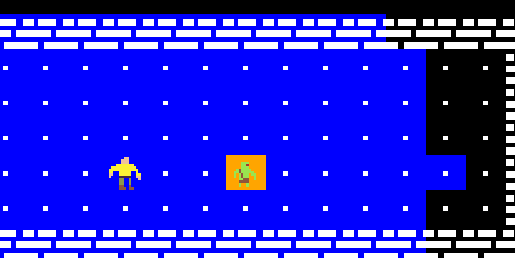
\includegraphics[width=8cm]{images/mygame/targeting.png}
	\caption{Wybór celu magicznego zwoju}
	\label{mygame:targeting}
\end{figure}
\FloatBarrier

\FloatBarrier
\begin{figure}[ht]
	\centering
	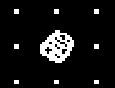
\includegraphics[width=3cm]{images/mygame/scroll.png}
	\caption{Magiczny zwój w grze}
	\label{mygame:scroll}
\end{figure}
\FloatBarrier

Dostępne w grze zwoje to: 
\begin{itemize}
	\item 'Magic missile scroll' -- magiczny pocisk, zadaje obrażenia wybranemu celowi;
	\item 'Fireball scroll' -- ognista kula, zadaje obrażenia przeciwnikom w małym promieniu od wybranego celu;			
	\item 'Sleep scroll' -- uśpienie, usypia wybrany cel na kilka tur -- nie będzie się on poruszał ani atakował;
	\item 'Area sleep scroll' -- uśpienie obszarowe, usypia kilka przeciwników w małym promieniu od wybranego celu;
	\item 'Teleport scroll' -- teleportacja, natychmiast przenosi postać gracza w wybrane miejsce.	
\end{itemize}


\subsection{Tester proceduralnie generowanych poziomów}
Gry roguelike opierają się w głównej mierze na proceduralnie generowanych poziomach, co oznacza generowanie map na podstawie algorytmów zawierających elementy losowości. Znaczy to na przykład, że użyty w niniejszej grze algorytm do generowania jaskiń zawsze wygeneruje poziom przypominający jaskinię, lecz za każdym razem inaczej wyglądający. Takie podejście do tworzenie poziomów pozwala znacznie zaoszczędzić czas, który w standardowej metodzie byłby spędzony na ręcznie tworzenie poziomów. Mapy proceduralnie generowane są jednak podatne na błędy -- na przykład generowane są miejsca, do których nie da się dojść. W celu szybszego odnajdywania i naprawiania takich i podobnych pułapek, a także prezentacji możliwości zaimplementowanych algorytmów stworzono menu do testowania generatorów map, zaprezentowane na rysunku \ref{mygame:gen_test}. Opcja ta dostępna jest w głównym menu gry po wybraniu 'Test Map Generators'.

\FloatBarrier
\begin{figure}[ht]
	\centering
	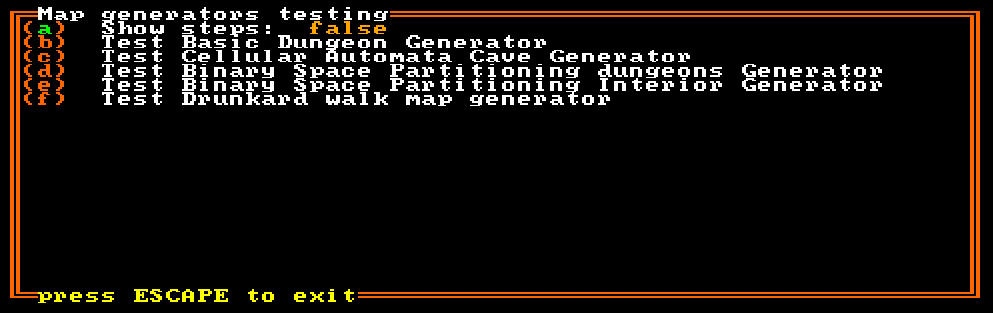
\includegraphics[width=14cm]{images/mygame/gen_test.png}
	\caption{Menu testera proceduralnie generowanych map}
	\label{mygame:gen_test}
\end{figure}
\FloatBarrier

Klawiszami strzałek oraz klawiszem Enter wybiera się opcję, klawiszem Esc można powrócić do głównego menu gry. Opcje dostępne w menu to:

\begin{enumerate}[label=\alph*), leftmargin=1.25cm]
	\item 'Show steps' -- zmiana opcji pokazania kroków generacji w trakcie testowania generatorów. 'true' oznacza włączenie pokazu kroków, 'false' wyłączenie,
	\item 'Test Basic Dungeon Generator' -- testowanie generacji poziomu 1,			
	\item 'Test Cellular Automata Cave Generator' -- testowanie generacji poziomu 3,
	\item 'Test Binary Space Partitioning dungeons Generator' -- testowanie generacji poziomu 2.
	\item 'Test Binary Space Partitioning Interior Generator' -- testowanie generacji poziomu 5.
	\item 'Test Drunkard walk map generator' -- testowanie generacji poziomu 4.
\end{enumerate}

Po wybraniu generatora map otwiera się okno zaprezentowane na rysunku \ref{mygame:window_tester}. W głównej części zaprezentowany jest aktualny stan mapy w przypadku pokazu z krokami lub finalny efekt generacji planszy w przypadku wyłączenia kroków. W dolnej części okna znajdują się informacje o numerze aktualnego kroku oraz jego opisie. Klawiszem Esc powrócić można do menu testera, klawiszem spacji generuje się nową mapę lub przechodzi do kolejnego kroku.

\FloatBarrier
\begin{figure}[ht]
	\centering
	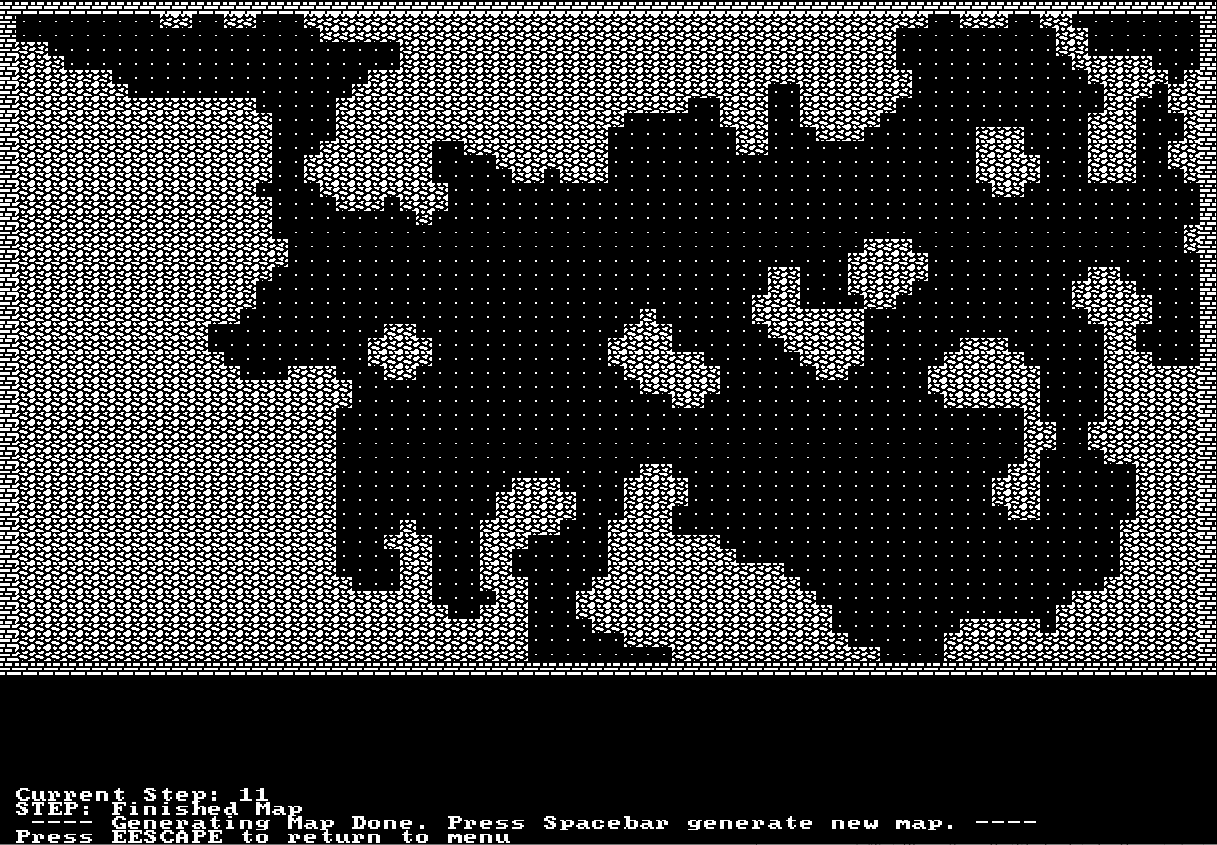
\includegraphics[width=14cm]{images/mygame/window_tester.png}
	\caption{Okno testera wybranego generatora map}
	\label{mygame:window_tester}
\end{figure}
\FloatBarrier

Na rysunku \ref{mygame:tester_steps} przedstawiono część kroków generacji mapy do poziomu trzeciego, na rysunku \ref{mygame:tester_nosteps} pokazano przykładowe wygenerowane mapy do poziomu drugiego.

\FloatBarrier
\begin{figure}[ht]
	\centering
	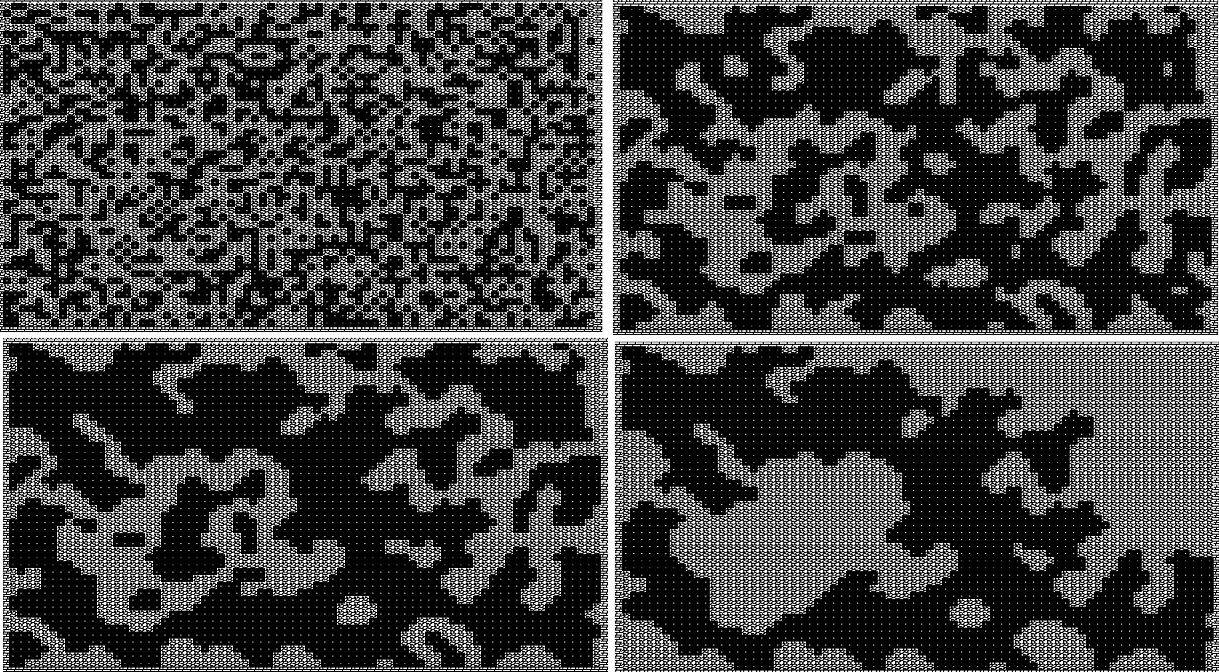
\includegraphics[width=16cm]{images/mygame/tester_steps.png}
	\caption{Przykład testowania z krokami generacji mapy do poziomu trzeciego}
	\label{mygame:tester_steps}
\end{figure}
\FloatBarrier

\FloatBarrier
\begin{figure}[ht]
	\centering
	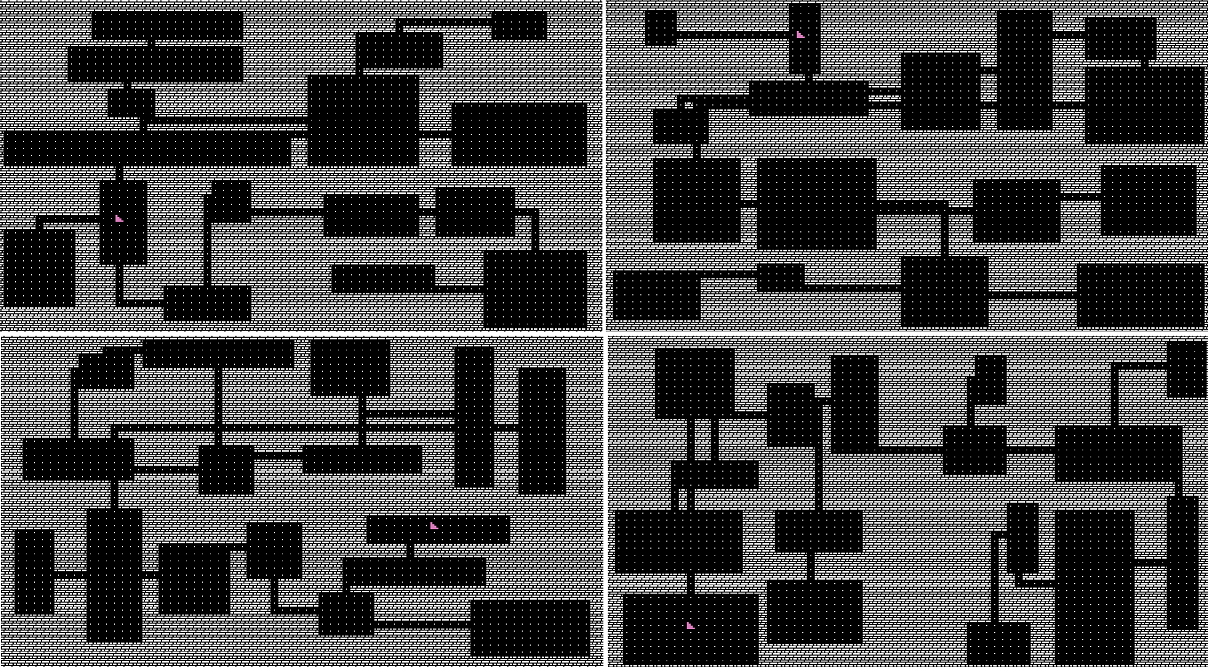
\includegraphics[width=16cm]{images/mygame/tester_nosteps.png}
	\caption{Przykład testowania bez kroków generacji mapy do poziomu drugiego}
	\label{mygame:tester_nosteps}
\end{figure}
\FloatBarrier

\clearpage	



\section{Technologie i implementacja}
W niniejszym rozdziale opisano technologie, architekturę oraz algorytmy użyte do implementacji gry. W ostatnim podrozdziale szczegółowo omówiono użyte metody proceduralnego generowania map.


\subsection{Technologie}
Do zaprogramowania gry użyto języka Rust, będącego kompilowalnym językiem ogólnego przeznaczenia, powstałym w 2010 roku \cite{book_rust}. Język Rust wydajnościowo jest porównywalny do języka C++, lecz jest to język nowocześniejszy i bezpieczniejszy \cite{rust_vs_cpp}. Język jest dużo bardziej restrykcyjny już na poziomie kompilacji, dzięki czemu błędy są częściej wykrywane w trakcie kompilacji, niż dopiero po uruchomieniu programu. Użyto też wbudowanych w język narzędzi: 'cargo fmt' do formatowania oraz 'cargo clippy' wyszukującego niegroźne błędy niewykrywalne przez kompilator, ale utrudniające czytelność kodu. Te cechy oraz narzędzia języka Rust znacznie ułatwiają stosowanie zasad czystego kodu \cite{book_czystykod}.

Do edycji kodu użyty został program Visual Studio Code \cite{vs_code} z rozszerzeniami dla języka Rust, przede wszystkim 'rust-analyzer` zapewniający kolorowanie składni, oraz automatyczne uzupełnianie kodu.

W programie użyto wielu tworzonych przez społeczność bibliotek open source -- zapewniających prawo do korzystania, oraz dostęp do kodu źródłowego. Najważniejsze użyte biblioteki to:
\begin{itemize}
	\item `rltk` -- tworzenie okna gry, obsługa grafiki oraz pętli głównej gry,
	\item 'specs' -- implementacja architektury Entity Component System.
\end{itemize}

Gra posiada grafikę typu \emph{pixel art} w formacie 16x16 pikseli. W oknie gry użyto dwukrotnie powiększonych obrazków w formacie 32x32 w celu polepszenia widoczności. Aby móc zmieścić całą mapę w jednym oknie w testerze proceduralnych generatorów map, użyty został oryginalny format 16x16. Do tworzenia grafiki użyto programu Aseprite \cite{aseprite} będącego wygodnym narzędziem graficznym wyspecjalizowanym w tworzeniu grafiki \emph{pixel art}. Wszystkie obrazki użyte w grze znajdują się w folderze 'resources' w dwóch plikach, odpowiednio 'sprite\_sheet\_16x16.png' oraz 'sprite\_sheet\_32x32.png'. Taki format przechowywania obrazków zapewnia porządek w folderach gry. Dostęp do konkretnego obrazka odbywa się przez określenie wymiarów oraz podaniu indeksu. Aby uzyskać obrazek przedstawiający gracza z pliku 'sprite\_sheet\_16x16.png' przedstawionego na rysunku \ref{mygame:spritesheet} należy określić rozmiary -- 16x16 pikseli oraz podać indeks 2 -- obrazki są indeksowane od lewej do prawej, pierwszy element ma indeks zero.

\FloatBarrier
\begin{figure}[ht]
	\centering
	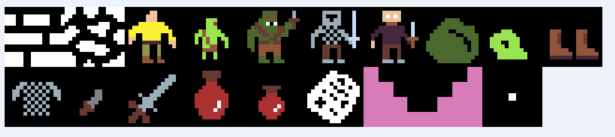
\includegraphics[width=12cm]{images/mygame/spritesheet.png}
	\caption{Grafiki użyte w grze. Od lewej: ściana, skały, postać gracza, goblin, ork, rycerz, łotr, szlam, mały szlam, buty, zbroja, sztylet, miecz, duża mikstura zdrowia, mikstura zdrowia, magiczny zwój, schody w dół, schody w górę, podłoga}
	\label{mygame:spritesheet}
\end{figure}
\FloatBarrier

\subsection{Implementacja}
W niniejszym podrozdziale przedstawiono szczegóły implementacji, wraz z prezentacją fragmentów kodu źródłowego wybranych elementów gry.


\subsubsection{Struktura projektu}
Gra posiada wiele modułów spełniających odmienne zadania. Kod projektu podzielony został na wiele modułów i pod-modułów w celu lepszej organizacji. Główny folder programu zawiera foldery: 'resources' -- zawierający grafiki użyte w grze oraz 'src' -- zawierający kod źródłowy. Na rysunku \ref{code:main_structure} przedstawiono schemat głównych modułów kodu projektu. W folderze głównym znajduje się też plik Cargo.toml określający między innymi użyte biblioteki.

\begin{figure}[ht]
	\centering
	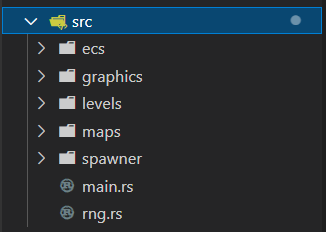
\includegraphics[width=12cm]{images/code/main_structure.png}
	\caption{Schemat głównych modułów struktury projektu}
	\label{code:main_structure}
\end{figure}
\FloatBarrier

Moduł 'ecs' zawiera podstawowy plik projektu 'game\_state.rs' obsługujący główną pętlę gry jako maszyna stanów. W tym module znajdują się też pod-moduły:
 
 \begin{itemize}
 	\item 'components' -- definicje komponentów,
 	\item 'systems' -- zawiera systemy, dzieli się na kolejne pod-moduły: 
 	\begin{itemize}
 		\item 'ai' -- systemy sterujące komputerowymi przeciwnikami;
 		\item 'combat' -- systemy związane z walką i zadawaniem obrażeń;
 		\item 'effects' -- efekty takie jak leczenie i teleportacja;
 		\item 'inventory' -- systemy zarządzania ekwipunkiem, podnoszenia i używania przedmiotów;
 		\item 'map' -- systemy związane z mapą;
 		\item 'player' -- systemy poruszania i akcji postaci gracza, oraz odczytywania wciśniętych klawiszy;
 		\item 'spawn' -- system umieszczania obiektów na poziomie,;
 		/item 'view\_system' -- system obliczania pola widzenia gracza oraz przeciwników.
 	\end{itemize}
 \end{itemize}
 
Moduł 'graphics' odpowiada za grafikę: tworzenie okna gry, rysowanie mapy i okien interfejsu. Znajdują się w nim funkcje do rysowania mapy gry, oraz obiektów: przedmiotów i postaci. Posiada pod-moduł 'menus' z definicją struktur odpowiedzialnych za poszczególne okna w grze, a także definicję cechy `WindowOptionSelector`, która implementuje większość tych struktur.

Moduł 'levels' posiada definicję struktury 'Level' odpowiedzialnej za poziom, oraz 'LevelManager' odpowiedzialnej za przechowywanie i tworzenie nowych poziomów.

W module 'map' zdefiniowana jest struktura przechowująca kształt mapy: 'Map', definicja typów pól na mapie oraz pomocnicze funkcje związane z mapą. Zawiera też pod-moduł 'generators' zawierający generatory poszczególnych typów map.

Moduł 'spawner' jest odpowiedzialny za tworzenie obiektów w grze takich jak: postać gracza, przeciwnicy oraz przedmioty. Zawiera też definicję struktur 'SpawnTable` odpowiadających za rozmieszczanie obiektów na konkretnych poziomach.

Plik 'main.rs' zawiera funkcję główną programu: 'main()'. W tej funkcji deklaruje się podstawowe konfigurację takie jak rozmiary map i okna gry, a także uruchamiana w niej jest pętla główna gry.
 
W pliku 'rng.rs' zawarto funkcje do losowania liczb używane w generatorach map, a także przy rozmieszczaniu na nich przeciwników i przedmiotów.

\subsubsection{Architektura Entity Component System}
Twórcy gier gatunku roguelike dzięki prostej grafice mogą poświęcić więcej czasu na tworzenie skomplikowanych i interesujących mechanik. Szczególnie przydatną w tworzeniu takich skomplikowanych mechanik jest architektura Entity Component System (Encja, Komponent, System), nazywana dalej ECS \cite{ecs_source}, skupiająca się na rozdzieleniu danych od systemów. Dzięki użyciu biblioteki 'specs' pominięto etap implementowania architektury ECS a skupiono się wyłącznie na jej użyciu.

Elementami ECS są :
\begin{itemize}
	\item 'Entity' -- encja, jest to indeks reprezentujący dany obiekt w grze na przykład gracza, przeciwnika lub przedmiot,
	\item 'Component' -- komponent, są to części składowe obiektów w grze przypisywane do konkretnych encji,
	\item 'System' -- części logiczne architektury, konkretne systemy aktualizują stany konkretnych komponentów,
	\item w niektórych implementacjach stosowany też jest czwarty element 'Event' -- wydarzenie, służący do informowania konkretnych obiektów o takich wydarzeniach jak na przykład zadanie obrażeń lub użycie przedmiotu. W przypadku tej gry wydarzenie zostały zrealizowane za pomocą odpowiednich komponentów.
\end{itemize}
	
Komponenty to małe części składowe, których stan aktualizowany jest przez konkretne systemy. Komponenty tworzone są jako struktury implementujące cechę 'Component' z biblioteki 'specs'. Definicje komponentów znajdują się w pliku 'src/ecs/components/mod.rs'. Przykładowe komponenty przedstawione na rysunku \ref{code:comps} to:
\begin{itemize}	
	\item 'BlocksTile' -- struktura bez pól, informuje, że dany obiekt blokuje aktualnie zajmowane pole i nie może się na nim znaleźć inny obiekt posiadający 'BlocksTile',
	\item 'Hp' -- informuje o maksymalnej i aktualnej liczbie punktów zdrowia. Posiadacze tego komponentu mogą zostać zranieni,
	\item 'CombatBaseStats' -- statystyki bojowe: atak i obrona, informują odpowiednio o ilości zadawanych obrażeń w trakcie walki i o ilości blokowanych obrażeń,
	\item 'WantsToMeleeAtack' -- komponent-wydarzenie dodawany do obiektu chcącego dokonać ataku, informuje o celu ataku,
	\item 'SufferDamage' -- komponent-wydarzenie dodawany do obiektów, którym zadane zostały obrażenia. Ilości obrażeń przedstawione są jako wektor, gdyż w jednej turze jeden obiekt może zostać zaatakowany przez kilku przeciwników.
\end{itemize}
	
\FloatBarrier
\begin{figure}[ht]
	\centering
	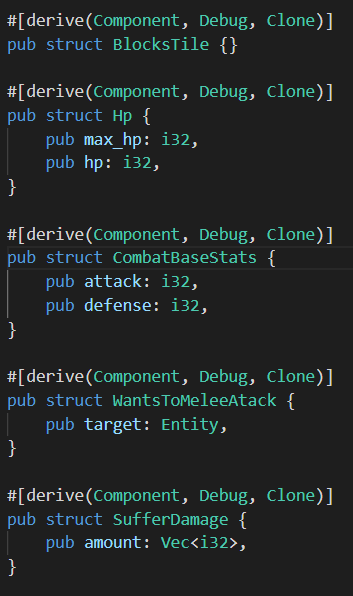
\includegraphics[width=8cm]{images/code/comps.png}
	\caption{Przykładowe struktury komponentów}
	\label{code:comps}
\end{figure}
\FloatBarrier

Na rysunku \ref{code:spawn_player} pokazano przykładowe tworzenie encji za pomocą przydzielania jej odpowiednich komponentów. Tworzoną encją w tym przypadku jest postać gracza. Poniżej wyjaśniono znaczenie komponentów, z których składa się bohater, poza komponentami wyjaśnionymi wcześniej:
\begin{itemize}	
	\item 'Player' -- struktura bez pól, informuje, że dany obiekt jest sterowany przez gracza. W grze powinien istnieć dokładnie jeden obiekt posiadający ten komponent;
	\item 'Movable' -- obiekt z tym komponentem jest w stanie się poruszać. Zawiera on kierunek kolejnego ruchu lub 'None' w przypadku braku ruchu;
	\item 'View' -- obiekt posiadający ten komponent posiada wzrok. Określa zasięg widzenia oraz aktualnie widziane pola na mapie;
	\item 'ViewMemory' -- pozwala zapamiętywać zobaczone wcześniej pola na mapie. Zawiera listę odkrytych już pól,
	\item 'Position' -- obiekt może zajmować określoną w tym komponencie pozycję na mapie;
	\item 'Name' -- określa nazwę danego obiektu;
	\item 'Renderable' -- obiekt z tym komponentem posiada przypisaną do niego grafikę i może być rysowany na mapie,
	\item 'BodyParts' -- obiekt posiada części ciała na które może założyć ekwipunek. 'default\_humanoid()' to domyślne części ciała dla postaci o ciele podobnym do ludzkiego: głowa, tors, ręce i nogi;
	\item 'Inventory' -- pozwala obiektowi na podnoszenie i przechowywanie przedmiotów.
\end{itemize}

\FloatBarrier
\begin{figure}[ht]
	\centering
	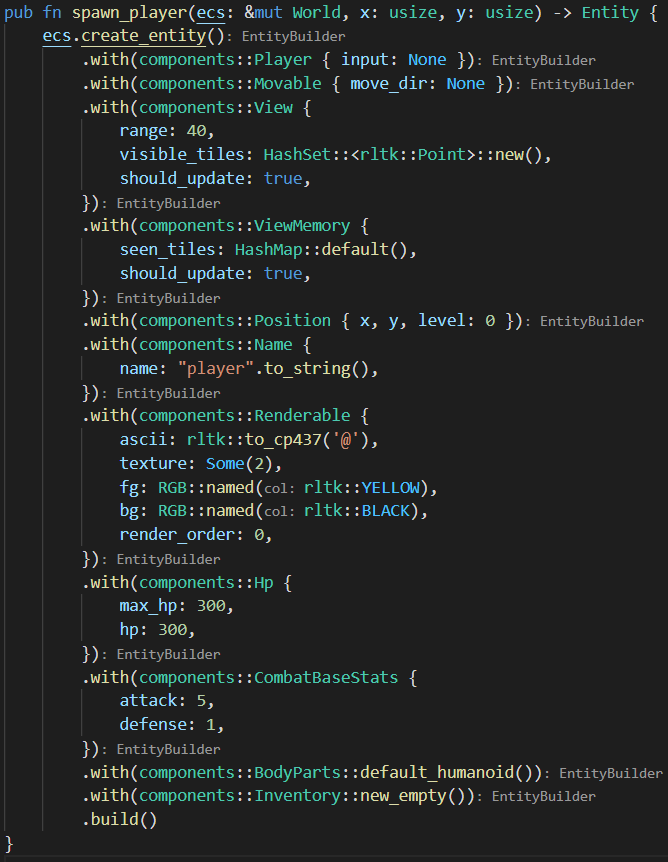
\includegraphics[width=12cm]{images/code/spawn_player.png}
	\caption{Funkcja tworząca encję gracza i przydzielająca mu odpowiednie komponenty}
	\label{code:spawn_player}
\end{figure}
\FloatBarrier


Systemy odpowiedzialne są za logikę gry, ich celem jest aktualizacja konkretnych komponentów. Na rysunku \ref{code:system_damage} przedstawiono system odpowiedzialny za przyjmowanie obrażeń. Systemy utworzone są jako puste struktury implementujące cechę 'System' z biblioteki specs. W implementacji tej cechy najpierw zdefiniowano typ 'SystemData' określający do jakich danych oraz w jaki sposób ma dostęp. Dla tego systemu przyznano dostęp do komponentów 'Hp' i 'SufferDamage'. Następnie zdefiniowano funkcję 'run' wymaganą przez cechę 'System;. W pierwszej linijce funkcji utworzono zmienne 'hps' - zbiór wszystkich komponentów 'Hp' oraz 'damages' - zbiór wszystkich komponentów 'SufferDamage'. Użyta w pętli for funkcja 'join' wyodrębnia komponenty znajdujące się na wszystkich zbiorach, na których została ona wywołana oraz gdzie komponenty te przypisane są do wspólnego właściciela -- Encji. Oznacza to, że każda iteracja pętli posiada dostęp do konkretnych komponentów ze zbiorów przekazanych do tej funkcji będących komponentami jednej Encji. Dla każdej Encji, która posiada te dwa komponenty odjęto sumę przyjętych obrażeń od aktualnego poziomu życia. Z racji, że komponenty 'SufferDamage' są komponentami-wydarzeniami, to można je usunąć po skończeniu pętli.

\FloatBarrier
\begin{figure}[ht]
	\centering
	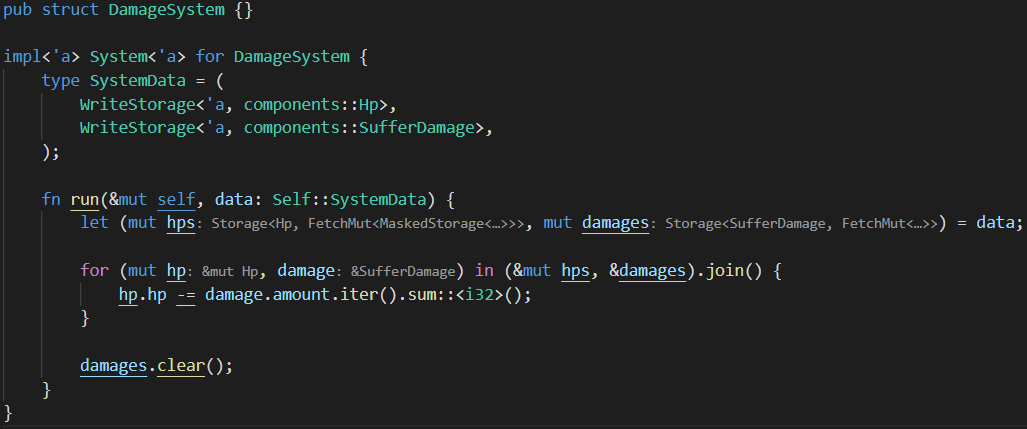
\includegraphics[width=16cm]{images/code/system_damage.png}
	\caption{System 'DamageSystem' odpowiedzialny za zadawanie obrażeń obiektom}
	\label{code:system_damage}
\end{figure}
\FloatBarrier

W przypadku systemów ważna jest kolejność ich wywoływania. W trakcie tury przeciwników najpierw wywoływany jest system `AISystem` odpowiedzialny za akcje przeciwników komputerowych. Następnie zadawane są obrażenia za pomocą 'MeleeCombatSystem`, oraz omówionego wcześniej 'DamageSystem`. Na końcu uruchamiana jest funkcja `delete\_the\_dead` odpowiedzialna za usuwanie postaci, których punkty życia osiągnęły zero.

\subsubsection{Pętla główna gry oraz jej stany}
Za stan gry odpowiada struktura 'State' z pliku 'game\_state.rs'. Implementuje ona funkcję `tick()`, która uruchamiana jest w nieskończonej głównej pętli gry. Działanie funkcji 'tick' zależne jest od aktualnego stanu gry opisanego za pomocą typu wyliczeniowego 'RunState`. Możliwe stany gry to:
\begin{itemize}
	\item 'MainMenu' -- wyświetlane jest menu główne gry;
	\item 'MapGenTesting(bool)' -- wyświetlane jest menu testera proceduralnie generowanych map. Ta opcja zawiera dodatkową zmienną typu bool, ustawienie tej zmiennej na true oznacza wyświetlanie testowanej mapy, false oznacza wyświetlenie menu testera;
	\item 'AwaitingInput' -- wyświetlane jest okno gry, gra oczekuje na akcję gracza;
	\item 'PreRun' -- uruchamiane są wszystkie podstawowe systemy gry, następny stan to 'AwaitingInput';
	\item 'PlayerTurn' -- uruchamiane są wszystkie podstawowe systemy gry, następny stan to 'MonsterTurn';
	\item 'MonsterTurn' -- uruchamiane są wszystkie podstawowe systemy gry, następny stan to 'AwaitingInput';
	\item 'ShowInventory' -- wyświetlane jest okno ekwipunku, gra oczekuje na akcję gracza;
	\item 'ShowEquipment' --wyświetlane jest okno aktualnie założonych zbrój i broni, gra oczekuje na akcję gracza;
	\item 'ShowItemActions(Entity)' -- wyświetlane jest okno akcji konkretnego przedmiotu, gra oczekuje na akcję gracza;
	\item 'Targeting(TargetingAction)' -- gracz określa cel dla konkretnego przedmiotu określonego w TargetingAction, określony też jest zasięg danego przedmiotu;
	\item 'MoveLevel(usize)' -- gracz przenosi się do poziomu o podanym indeksie. Jeśli poziom ten jeszcze nie istnieje, to 'LevelManager' go tworzy;
	\item 'GameOver' -- wyświetlane jest okno informujące o przegraniu gry, co ma miejsce w razie śmierci postaci gracza. Gra czeka na wciśnięcie konkretnego klawisza po którym wraca do menu głównego;
	\item 'Controls' -- wyświetlane jest okno informacji o sterowaniu;
	\item 'Won' -- wyświetlane jest okno informujące o wygraniu gry. Gra czeka na wciśnięcie konkretnego klawisza po którym wraca do menu głównego.
\end{itemize}

\subsubsection{System rozmieszczania przeciwników i przedmiotów na poziomach}
W grze występuje wiele rodzajów przeciwników i przedmiotów, a z racji generowaniu map w sposób proceduralny nie jest możliwe określenie ich statycznych położeń. W tym celu utworzono system określający jakie obiekty lub postacie występują na poziomach, oraz jakie są ich ilości oraz szansa wystąpienia. System ten został zdefiniowany w pliku 'spawner/spawn\_tables.rs' i składa się z następujących struktur w kolejności od najmniejszej części składowej: `SpawnEntry`, `SpawnPack` oraz `SpawnTable`.
 
Struktura 'SpawnEntry' przedstawiona na rysunku \ref{code:spawn_entry} składa się z pól:
\begin{itemize}
	\item 'entity\_name' -- nazwa obiektu. Nazwa ta musi być uwzględniona w funkcji `spawner/mod.rs/spawn\_entity()`, która odpowiada za umiejscowienie obiektu o danej nazwie na podanej pozycji,
	\item 'rng\_range' -- określa zasięg od minimalnej do maksymalnej liczby obiektów, które mogą zostać utworzone w ramach danego 'SpawnEntry'. Dokładna liczba jest losowana w podanym zakresie,
	\item 'chance\_perc' -- określa szansę w punktach procentowych na pojawienie obiektów z danego 'SpawnEntry'.	
\end{itemize}

 
\FloatBarrier
\begin{figure}[ht]
	\centering
	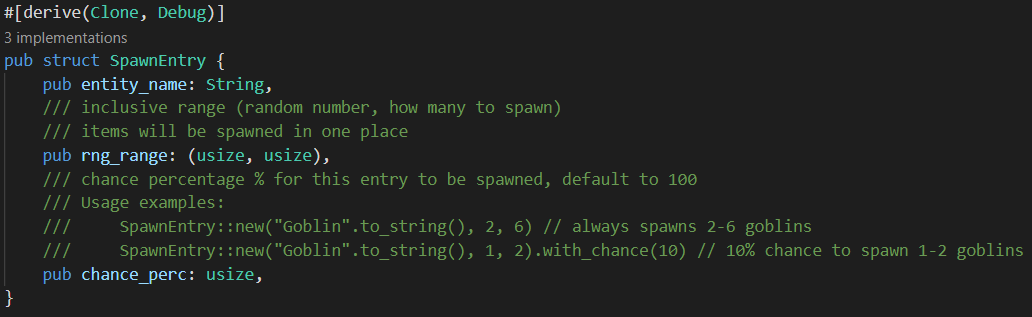
\includegraphics[width=16cm]{images/code/spawn_entry.png}
	\caption{Struktura 'SpawnEntry'}
	\label{code:spawn_entry}
\end{figure}
\FloatBarrier
 
Każdy generator map posiada metodę zwracającą dla wygenerowanej przez niego mapy, wydzielone obszary nazywane 'spawn areas'. Są to obszary, na których może pojawić się grupa obiektów zdefiniowana w strukturze 'SpawnPack' zaprezentowanej na rysunku \ref{code:spawn_pack}. Struktura ta określa minimalny obszar, na którym może pojawić się ta grupa, szansę wystąpienia tej grupy, oraz maksymalną liczbę grup tego typu na danym poziomie.
 
\FloatBarrier
\begin{figure}[ht]
	\centering
	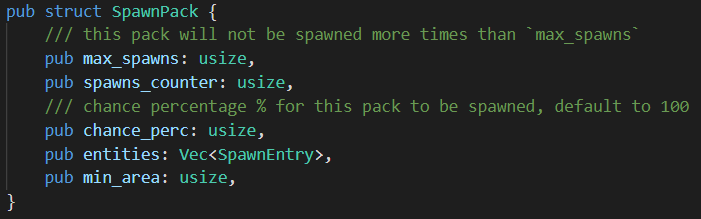
\includegraphics[width=16cm]{images/code/spawn_pack.png}
	\caption{Struktura 'SpawnPack'}
	\label{code:spawn_pack}
\end{figure}
\FloatBarrier

Na rysunku \ref{code:goblins_pack} przedstawiono funkcję tworzącą 'SpawnPack' będący grupą goblinów. W obszarze 'spawn area' dla którego wylosowana zostanie ta grupa, pojawi się od dwóch do sześciu goblinów, od zera do jednej mikstury życia, oraz zwój uśpienia z dwudziestoprocentową szansą na pojawienie się.

\FloatBarrier
\begin{figure}[ht]
	\centering
	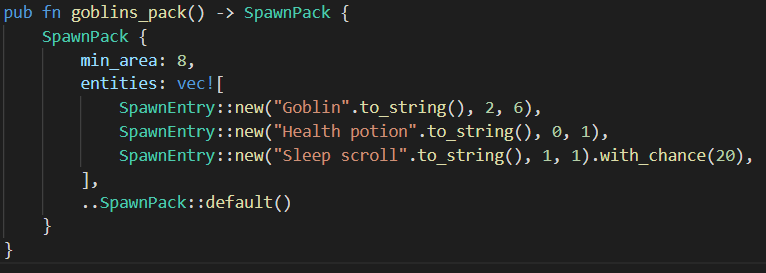
\includegraphics[width=16cm]{images/code/goblins_pack.png}
	\caption{'SpawnPack' grupa goblinów}
	\label{code:goblins_pack}
\end{figure}
\FloatBarrier

Ostatnim elementem rozmieszczania przedmiotów i przeciwników jest struktura 'SpawnTable' przedstawiona na rysunku \ref{code:spawn_table} , która określa możliwe do pojawienia się na danym poziomie grupy obiektów -- 'SpawnPack'. Na rysunku \ref{code:basic_spawn} przedstawiono tablicę możliwych grup na poziomie pierwszym.

\FloatBarrier
\begin{figure}[ht]
	\centering
	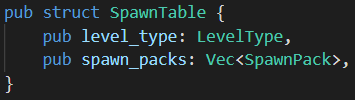
\includegraphics[width=6cm]{images/code/spawn_table.png}
	\caption{Struktura 'SpawnTable'}
	\label{code:spawn_table}
\end{figure}
\FloatBarrier

\FloatBarrier
\begin{figure}[ht]
	\centering
	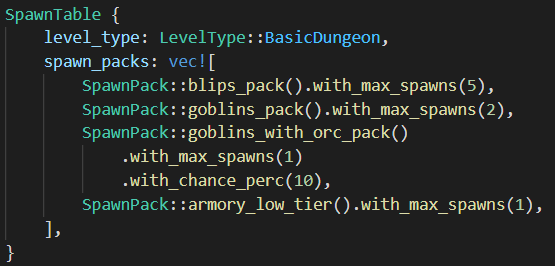
\includegraphics[width=10cm]{images/code/basic_spawn.png}
	\caption{Przykład 'SpawnTable' dla poziomu pierwszego}
	\label{code:basic_spawn}
\end{figure}
\FloatBarrier

Po skończeniu generacji poziomu, generator oblicza obszary 'spawn area'. Następnie dla każdego takiego obszaru losowana jest grupa 'SpawnPack' z tablicy 'SpawnTable' przypisanej dla danego poziomu. Losowanie to odbywa się do momentu gdy wszystkim obszarom zostanie przypisany 'SpawnPack', albo każdy z nich osiągnie maksymalną liczbę pojawień się. W każdej przypisanej grupie następują dwa losowania dla każdego 'SpawnEntry' składającego się na tą grupę. Wynik pierwszego losowania decyduje o pojawieniu się danych obiektów, a drugie określa ich liczbę. Każdy obiekt, który pojawił się w ramach danego 'SpawnPack' zostaje umieszczony na losowym miejscu w przypisanym do tej grupy obszarze 'spawn area'.


\subsection{Proceduralne generowanie poziomów}
Proceduralna generacja oznacza tworzenie poziomów na podstawie algorytmów z użyciem losowości. Oznacza to, że przy każdym generatorze, mapy przez niego tworzone będą różne, ale będą tego samego typu. Każdy generator posiada strukturę konfiguracyjną, dzięki czemu łatwo można zmieniać jego zasady, co w połączeniu z testerem proceduralnie generowanych map pozwala na szybkie dostosowywanie parametrów w celu osiągnięcia konkretnego wyglądu planszy. Przykłady wygenerowanych map pochodzą z testera generowania map.

\subsubsection{Poziom pierwszy}
Generator używany do tworzenia mapy poziomu pierwszego jest jednym z najprostszych i polega na stochastycznym rozmieszczeniu pokojów o losowych wymiarach. Pokoje nie mogą na siebie nachodzić, ich liczbę i rozmiar można określić w konfiguracji generatora. Po umieszczeniu na mapie poziomów są one łączone ze sobą korytarzami, w kolejności w jakiej się pojawiły.

\FloatBarrier
\begin{figure}[ht]
	\centering
	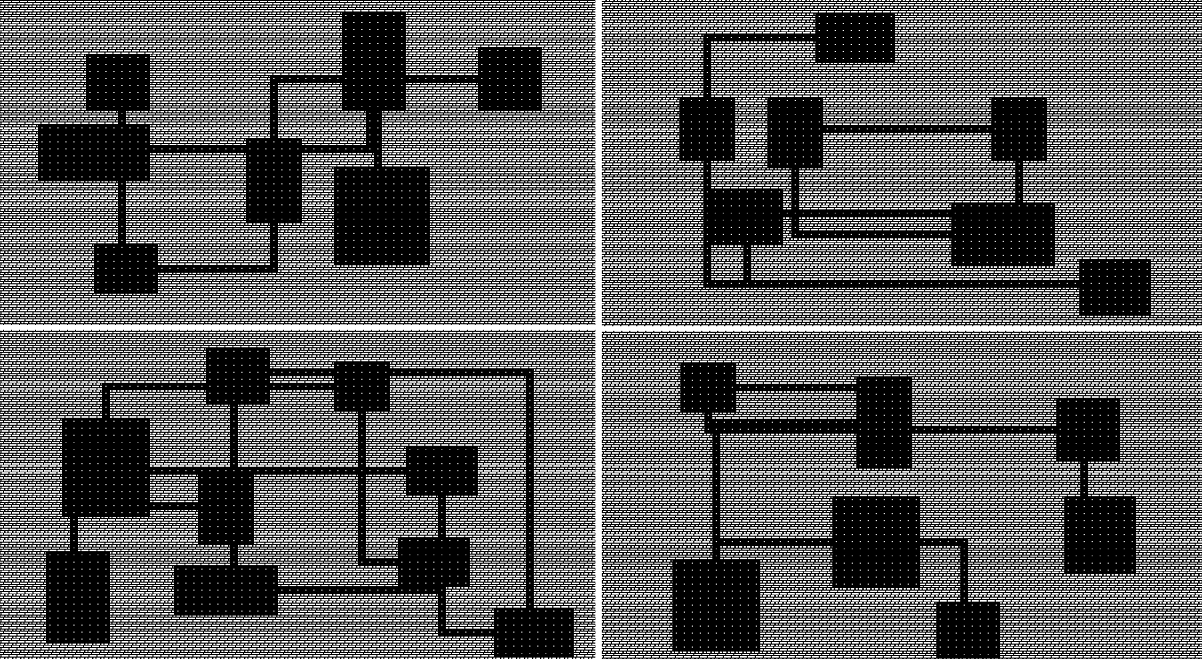
\includegraphics[width=10cm]{images/generators/level1.png}
	\caption{Przykład wygenerowanych map dla poziomu pierwszego}
	\label{generators:level1}
\end{figure}
\FloatBarrier


\subsubsection{Poziom drugi -- Binary Space Partitioning}
Generator użyty w poziomie drugim oparty jest o metodę Binary Space Partitioning \cite{bsp_source} -- binarne dzielenie przestrzeni, określane też za pomocą skrótu BSP. Metoda ta opiera się o drzewo binarne \cite{book_algo}, które zawiera kolejne pod-obszary mapy. Na rysunku \ref{generators:bsp_node} przedstawiono strukturę reprezentującą węzeł drzewa użytego w tej metodzie. Zawiera ona indeks węzła, poziom drzewa, na którym znajduje się ten węzeł, indeksy rodzica, siostry -- węzła o wspólnym bezpośrednim rodzicu, opcjonalne indeksy dzieci, indeksy kolejnych rodziców aż do korzenia, obszar zajmowany przez ten węzeł, oraz opcjonalnie obszar zajmowany przez pokój umieszczony w tym węźle.

\FloatBarrier
\begin{figure}[ht]
	\centering
	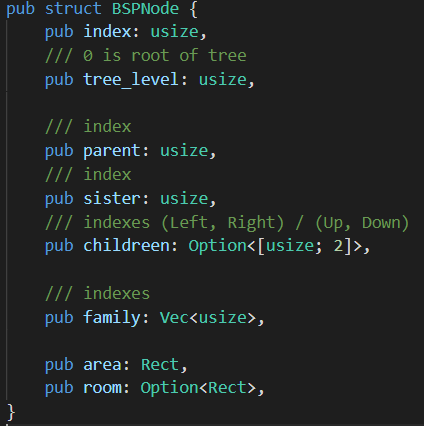
\includegraphics[width=10cm]{images/generators/bsp_node.png}
	\caption{Węzeł drzewa binarnego użyty w metodzie Binary Space Partitioning}
	\label{generators:bsp_node}
\end{figure}
\FloatBarrier

Korzeń drzewa zawsze zawiera obszar całej mapy. Następnie w losowym miejscu, zbliżonym do środka obecnego obszaru następuje podział na dwa obszary. Ten podział wykonywany jest losowo w sposób pionowy lub poziomy. Te dwa obszary są dziećmi obszaru, z którego się wywiodły. Taki podział następuje do momentu, gdy maksymalny, określony w generatorze poziom drzewa zostanie osiągnięty. Na rysunku \ref{generators:bsp_tree} przedstawiono przykładowy podział mapy na obszary z przypisaniem obszarów do węzłów drzewa. Liczby w każdym obszarze oznaczają jego rodzinę. Zapisana pierwsza liczba od prawej strony to indeks węzła zawierającego ten obszar, następnie w lewo indeks jego rodzica, indeks rodzica rodzica i tak dalej. Węzły z indeksem zaczynającym się od 15 to liście drzewa -- nie posiadają dzieci.

\FloatBarrier
\begin{figure}[ht]
	\centering
	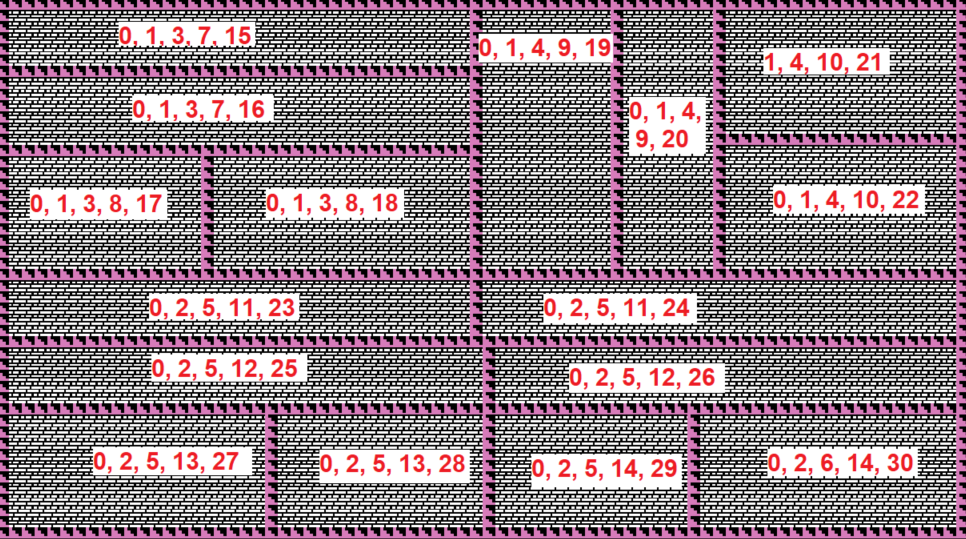
\includegraphics[width=14cm]{images/generators/bsp_tree.png}
	\caption{Przykład podziału map za pomocą metody Binary Space Partitioning}
	\label{generators:bsp_tree}
\end{figure}
\FloatBarrier

Następnie w każdym z obszarów zawartych w liściach drzewa umieszcza się pokój o losowych rozmiarach, przedstawiono to na rysunku \ref{generators:bsp_rooms}.

\FloatBarrier
\begin{figure}[ht]
	\centering
	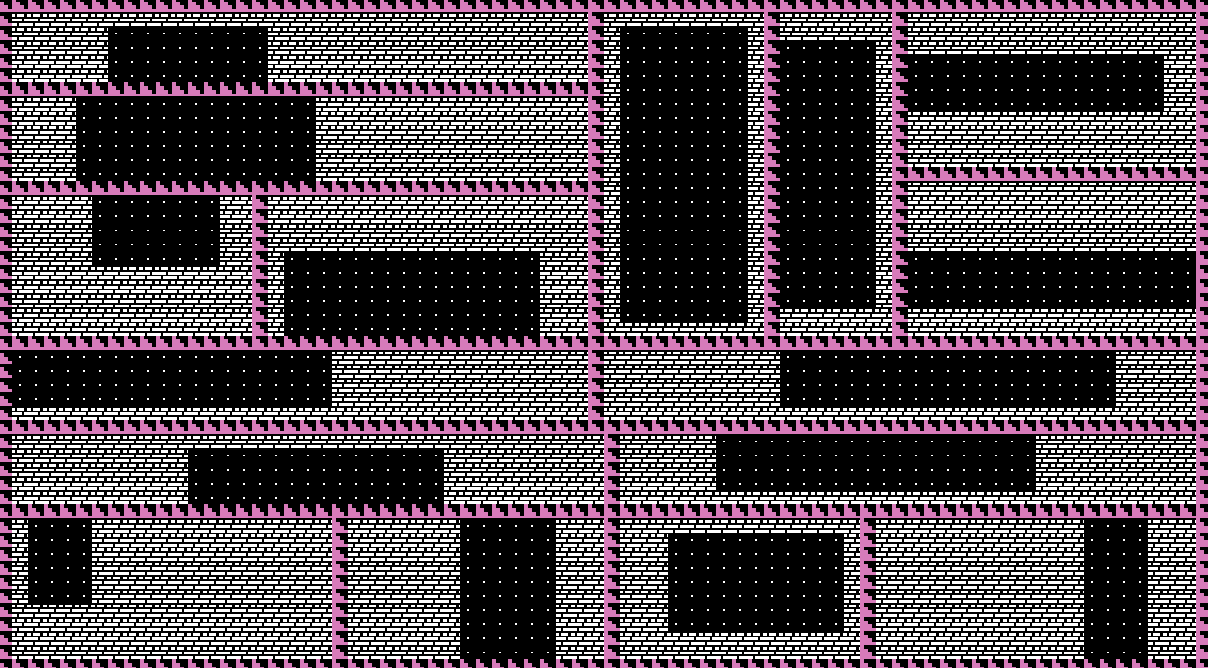
\includegraphics[width=12cm]{images/generators/bsp_rooms.png}
	\caption{Rozmieszczenie pokojów na mapie BSP}
	\label{generators:bsp_rooms}
\end{figure}
\FloatBarrier

Ostatnim krokiem jest połączenie ze sobą pokojów za pomocą korytarzy. Dzięki użyciu drzewa binarnego można zastosować lepsze rozwiązanie niż "każdy z każdym", zapewniające, że z każdego pokoju można w jakiś sposób dostać się do każdego innego. Przechodząc od przedostatniego poziomu drzewa w górę najpierw łączy się ze sobą po dwa pokoje znajdujące się w obszarach będących dziećmi węzłów z tego poziomu. W kolejnych poziomach dla każdego węzła wybiera się losowych potomków będących liśćmi z obojga dzieci każdego węzła danego poziomu i łączy się zawarte w nich pokoje. Po skończeniu tego procesu wszystkie pokoje są połączone w sposób, który zakłada, że na pewno istnieje połączenie między jednym z pokojów zawartych w obszarze węzła o indeksie 3 a jednym z pokojów z obszaru należącego do węzła 4, gdyż węzły o indeksach 3 i 4 są bezpośrednimi dziećmi węzła o indeksie 1. Na rysunku \ref{generators:bsp_done} można zaobserwować, że w omówionym powyżej przypadku połączony został pokój z liścia o indeksie 18 z pokojem z liścia o indeksie 19.

\FloatBarrier
\begin{figure}[ht]
	\centering
	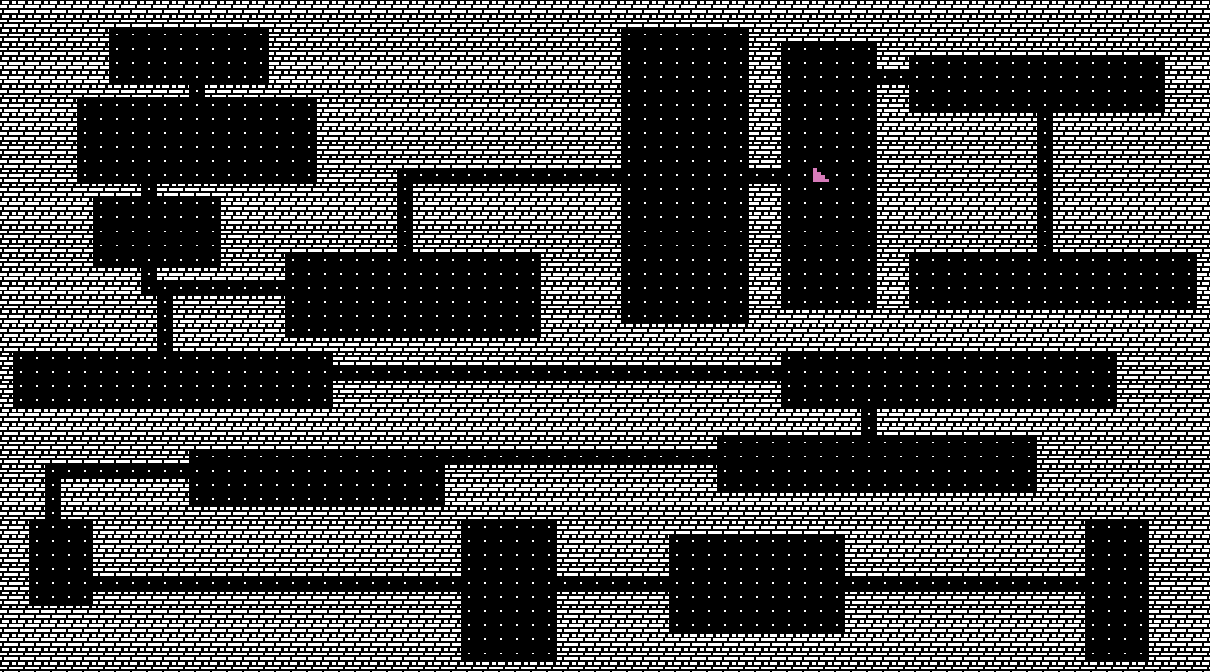
\includegraphics[width=14cm]{images/generators/bsp_done.png}
	\caption{Mapa wygenerowana za pomocą algorytmu binarnego podziału przestrzeni}
	\label{generators:bsp_done}
\end{figure}
\FloatBarrier


\subsubsection{Poziom trzeci -- Cellular Automata}
Generacja poziomu trzeciego oparta jest o automat komórkowy \cite{book_ca}, będący kwadratową siatką pól mogących być żywymi lub martwymi, których kolejny stan zależy od poprzedniego oraz od ustalonych warunków. W kreowaniu mapy za pomocą tej metody za żywe uznano pola będące podłogą, a za martwe pola będące ścianą. W pierwszym kroku każde pole na mapie w losowy sposób staje się żywe lub martwe. W kolejnych krokach o ustalonej liczbie, stan każdej komórki na mapie zmienia się według tego czy jest ona żywa czy martwa, oraz ilu posiada żywych sąsiadów -- pól stykających się z daną komórką. Opisują to następujące reguły:

\begin{itemize}
	\item jeśli komórka jest żywa oraz posiada mniej niż trzech żywych sąsiadów to w kolejnym kroku będzie martwa;
	\item jeśli komórka jest martwa i posiada więcej niż czterech żywych sąsiadów to w kolejnym kroku będzie żywa.
\end{itemize}

Ostatnim krokiem jest usunięcie wszystkich niepołączonych ze sobą obszarów, poza największym.

Za pomocą manipulowania zasadami tego algorytmu można w łatwy sposób zmieniać wygląd wygenerowanych plansz. Przykładowo na rysunku \ref{generators:ca_diff} po lewej stronie znajduje się mapa wygenerowana według standardowych zasad użytych w grze, a po prawej mapa, w której podłoga uznawana jest za martwą komórkę, a ściana za żywą.

\FloatBarrier
\begin{figure}[ht]
	\centering
	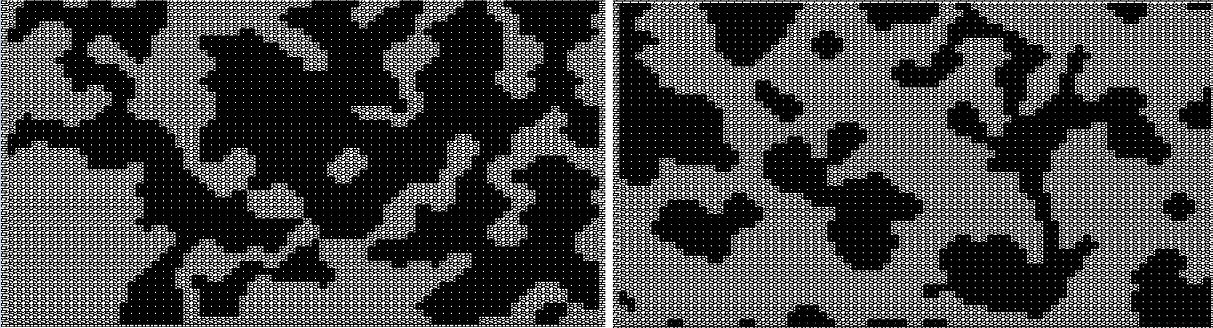
\includegraphics[width=16cm]{images/generators/ca_diff.png}
	\caption{Przykład manipulacji zasad algorytmu opartego o automat komórkowy}
	\label{generators:ca_diff}
\end{figure}
\FloatBarrier


\subsubsection{Poziom czwarty -- Drunkard Walk}
Generator map użyty w poziomie czwartym oparty jest o algorytm Drunkard Walk. W celu przystępniejszego wytłumaczenia zasad tego algorytmu posłużono się postacią górnika, który chodząc po planszy wykopuje kolejne pola, zamieniając je w podłogi. W implementacji użytej na potrzeby stworzonej gry, algorytm wykonuje się w następujących krokach:

\begin{itemize}
	\item wszystkie pola na mapie zamieniane są na ściany,
	\item następnie dopóki określona przestrzeń mapy nie będzie podłogą wykonuje się następujące kroki:
	\begin{enumerate}
		\item w centralnym polu mapy umieszcza się górnika;
		\item w określonej liczbie ruchów górnik porusza się o jedno pole w losowym kierunku a każde pole, po którym przejdzie zamienia się w podłogę;
		\item jeśli górnikowi skończyły się ruchy, a mapa wciąż nie zawiera określonej liczby miejsc nie będących ścianami algorytm powraca do kroku 1.
	\end{enumerate}	
\end{itemize}

W wyniku tego algorytmu otrzymać można mapy, których przykłady zaprezentowano na rysunku \ref{generators:drunkard_walk} 

\FloatBarrier
\begin{figure}[ht]
	\centering
	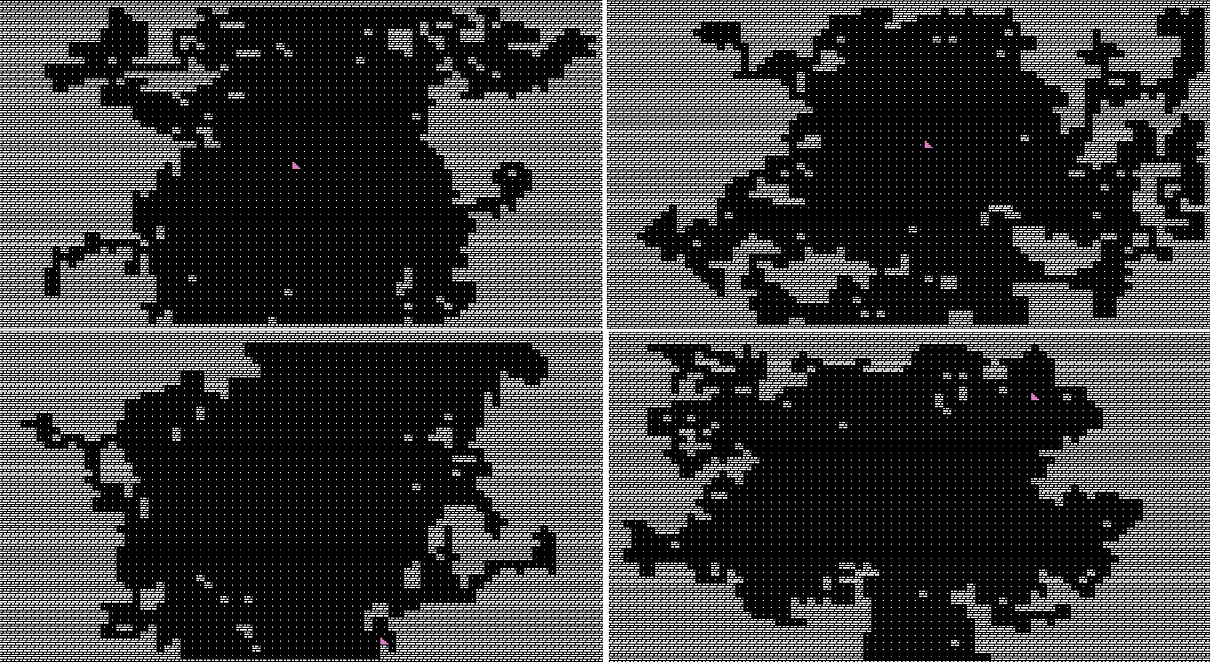
\includegraphics[width=16cm]{images/generators/drunkard_walk.png}
	\caption{Przykład działania generatora map opartego o algorytm Drunkard Walk}
	\label{generators:drunkard_walk}
\end{figure}
\FloatBarrier

\clearpage

\subsubsection{Poziom piąty -- Binary Space Partitioning}
Poziom piąty korzysta z tej samej metody Binary Space Partitioning, co poziom drugi, lecz pokoje w nim zajmują całe obszary przypisane do węzłów będących liśćmi drzewa. Pozwala to na wygenerowanie mapy podzielonej na pokoje bezpośrednio ze sobą połączone, bez użycia korytarzy. Na rysunku \ref{generators:bsp_diff} zaprezentowano porównanie mapy z poziomu drugiego z mapą z poziomu piątego.
	
\FloatBarrier
\begin{figure}[ht]
	\centering
	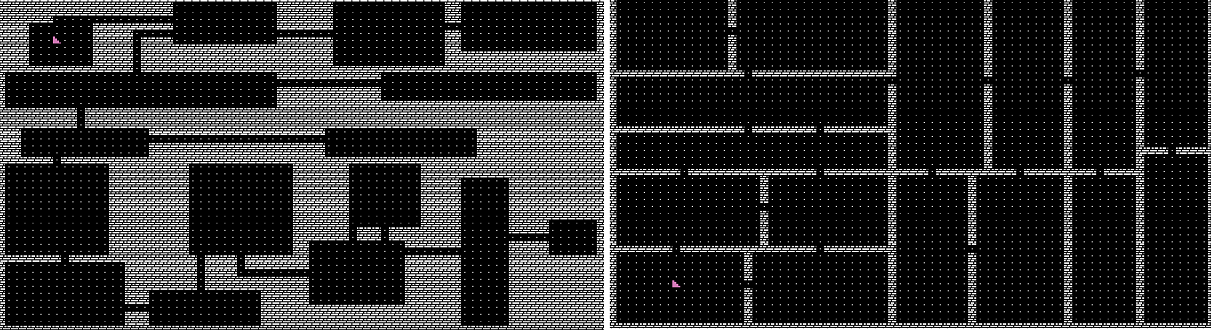
\includegraphics[width=16cm]{images/generators/bsp_diff.png}
	\caption{Porównanie map poziomu drugiego po lewej i piątego po prawej, wygenerowanych za pomocą metody BSP}
	\label{generators:bsp_diff}
\end{figure}
\FloatBarrier




\clearpage

\section*{Podsumowanie i wnioski końcowe}

Roguelike to gatunek, który z racji częstego używania losowości pozwala na interesującą i unikalną rozgrywkę. W niniejszej pracy pokazano, że mimo prostej grafiki i interfejsu, gry te mogą oferować ciekawe mechaniki rozgrywki oraz różnorodne, proceduralnie generowane poziomy. Gry tego typu nie są popularne, ale istnieją nowoczesne, bardziej popularne gry inspirujące się tym gatunkiem. \\ 


W ramach niniejszej pracy zrealizowane zostały założone cele: 
\begin{itemize}
	\item zaprogramowano grę roguelike o założeniach zgodnych z klasycznymi rozgrywkami tego gatunku;
	\item omówiono implementację mechanizmów rozgrywki;
	\item w grze użyte zostały mapy generowane w sposób proceduralny;
	\item omówiono różne metody użytych generatorów proceduralnych map.
\end{itemize}

Zrealizowano też dodatkowy cel pracy -- dokonanie charakterystyki porównawczej wybranych gier. Opisano grę uznawaną za pierwszą w gatunku roguelike -- Rogue, grę Caves of Qud będąca nowoczesnym rozwinięciem klasycznych rozgrywek oraz The Binding of Isaac -- grę implementującą wybraną część założeń gatunku. \\

Do gry wprowadzono nowe rozwiązania takie jak system testowania i prezentowania proceduralnie generowanych map, system rozmieszczania na mapach przeciwników i przedmiotów oparty o wydzielone obszary mapy oraz tablicę obiektów możliwych do pojawienia się na danym poziomie.
\\

Podczas realizacji pracy napotkano kilka problemów. Pierwszy z nich związany był z wyświetlaniem aktualnego stanu mapy w trakcie pracy generatora w celu prezentacji kroków proceduralnego generowania map. Aby tego dokonać konieczne było zapisywanie w trakcie generacji aktualnych stanów mapy w kluczowych momentach do wektora będącego historią generacji. W każdym generatorze zaimplementowano możliwość tworzenia takiej historii, którą mógł on zwrócić po skończeniu generowania mapy. Wyświetlenie kroków polegało później na wyznaczeniu kolejnych pozycji z tego wektora.

Kolejna trudność polegała na tym, iż użyty rozmiar map oraz rozmiar kwadratów na mapie 16x16 pikseli okazał się mało wyraźny, co tworzyło problemy w rozróżnieniu poszczególnych pól na mapie gry. Aby uniknąć zmiany rozmiarów map, które wcześniej dostosowane były do rozmiaru okna zastosowano w trakcie gry znaczne przybliżenie wycentrowane na postać gracza i użyto grafik w formacie 32x32 piksele. Aby tester generatorów map wciąż mógł być w stanie przedstawić całą mapę na ekranie gry zastosowano oryginalne grafiki 16x16. \\


Gra wykonana na potrzeby niniejszej pracy została napisana w sposób umożliwiający łatwą jej rozbudowę. Aplikację można rozbudować o następujące elementy:
\begin{itemize}
	\item większa liczba przedmiotów i ich efektów -- obecnie w grze nie ma wielu przedmiotów. Dodanie nowych ich typów z pewnością urozmaiciłoby rozgrywkę. Jako przykład można dodać mikstury zwiększające atak lub obronę bohatera na kilka tur;
	\item nowe metody generowania map -- pozwolą na dodanie do gry kolejnych poziomów, co przedłuży i urozmaici rozgrywkę. Możliwe jest też dodanie poziomów opartych o obecnie zaimplementowane metody, ale manipulując ich konfiguracją, lub używając kilku metod na jednej mapie;
	\item nowe typy przeciwników z interesującymi umiejętnościami -- obecnie przeciwnicy poza szlamem nie różnią się od siebie niczym poza wartościami obrony i ataku oraz ekwipunkiem. Interesującym dodatkiem do gry byliby przeciwnicy posiadający umiejętności, na przykład lodowy potwór mogący zamrozić gracza, przez co nie będzie on mógł się poruszać przez kilka tur;
	\item inteligentni przeciwnicy -- w aktualnej wersji gry przeciwnicy mogą tylko podążać za graczem, jeśli jest on w ich polu widzenia oraz atakować go, jeśli są bezpośrednio obok niego. Bardziej interesującym podejściem byłoby dodanie przeciwników, którzy nie zaatakują gracza, dopóki sami nie zostaną zaatakowani; przeciwnicy mogliby też uciekać przed graczem, jeśli zostanie im bardzo mało punktów zdrowia.
\end{itemize}


\clearpage



\addcontentsline{toc}{section}{Literatura}

\begin{thebibliography}{4}
	
% zrodlo film: Autor filmu [osoba/firma], tytuł, nazwa konferencji i odnośnik www.
% zrodlo gra : Autor gry [osoba/firma], nazwa gry i strona internetowa.

% ksiazka o komputerowych grach RPG
\bibitem{book_rpg} Felipe Pepe, The CRPG Book: A Guide to Computer Role-Playing Games, Bitmap Books, 2020.

% o roguelikach ogolnie https://www.routledge.com/Exploring-Roguelike-Games/Harris/p/book/9780367482596
\bibitem{bookroguelike} Harris J.: Exploring Roguelike Games. CRC Press, 2020.

% popularnosc nowoczesnych roguelike-ow
\bibitem{roguelike_popularity} Daniel Doan, Why Are Modern Roguelike Games So Popular?, https://gamedevlibrary.com/gamedev-thoughts-why-are-modern-roguelike-games-so-popular-53c1f5a05485.

% gra rogue (nie posiada oficjalnej strony)
\bibitem{rogue_game} Michael Toy, Glenn Wichman, Ken Arnold, Rogue, 1980, https://www.mobygames.com/game/rogue

% ksiazka o kodowaniu ascii
\bibitem{book_ascii} American Standards Association, American Standard Code for Information Interchange ASCII, 1963

% oficjalna strona gry caves of qud
\bibitem{game_coq} Freehold Games, Caves of Qud, 2015, https://www.cavesofqud.com

% artykul o pixel art
\bibitem{source_pixelart} Angie Kordic, What Exactly is Pixel Art and How Did It Come Back to Life ?, https://www.widewalls.ch/magazine/pixel-art

% oficjalna strona gry the binding of isaac
\bibitem{game_tboi} Edmund McMillen, Nicalis, The Binding of Isaac: Rebirth, 2014, https://bindingofisaac.com

% prezentacja o użyciu wave function collapse w Caves of Qud
\bibitem{coq_wfc} Brian Bucklew (Freehold Games), Math for Game Developers: Tile-Based Map Generation using Wave Function Collapse in 'Caves of Qud', Game Developers Conference, https://www.gdcvault.com/play/1026263/Math-for-Game-Developers-Tile .

% github wfc
\bibitem{wfc_git} https://github.com/mxgmn/WaveFunctionCollapse .

% prezentacja o proceduralnej historii w Caves of Qud
\bibitem{coq_history} Jason Grinblat (Freehold Games), Procedurally Generating History in 'Caves of Qud', Game Developers Conference, https://www.gdcvault.com/play/1024990/Procedurally-Generating-History-in-Caves .

% Caves of qud w serwisie Steam
\bibitem{coq_steam} https://store.steampowered.com/app/333640/Caves\_of\_Qud/


%The binding of isaac w serwisie Steam
\bibitem{tboi_steam} https://store.steampowered.com/app/250900/The\_Binding\_of\_Isaac\_Rebirth/

% gra planszowa na podstawie tboi zebrala milion w tydzien
\bibitem{tboi_4souls} Stefanie Fogel, ‘The Binding of Isaac’ Card Game Surpasses 1 Million on Kickstarter in Just Over a Week, https://variety.com/2018/gaming/news/the-binding-of-isaac-four-souls-kickstarter-1202868455/


% ksiazka Rust
\bibitem{book_rust}  Steve Klabnik , Carol Nichols, The Rust Programming Language, No Starch Press, 2019.

% rust vs c++
\bibitem{rust_vs_cpp} Ben Fenwick, C++ v. Rust -Speed, Safety, \& Community Comparison, https://devetry.com/blog/c-v-rust-speed-safety-community-comparison/ .

% czysty kod
\bibitem{book_czystykod} Robert C. Martin, Czysty kod. Podręcznik dobrego programisty, Helion, 2014.

% vs code
\bibitem{vs_code} Microsoft, Visual Studio Code, 2015, https://code.visualstudio.com .

% program do pixel art
\bibitem{aseprite} Igara Studio S.A, Aseprite, 2001, https://www.aseprite.org.

% artykul o ECS
\bibitem{ecs_source} Richard Lord, Why use an Entity Component System architecture for game development?, https://www.richardlord.net/blog/ecs/why-use-an-entity-framework.html .

% mapy bsp
\bibitem{bsp_source} http://www.roguebasin.com/index.php/Basic\_BSP\_Dungeon\_generation .

% algorytmy i struktury danych
\bibitem{book_algo} Alfred V. Aho, John E. Hopcroft, Jeffrey D. Ullman, Algorytmy i struktury danych, Helion 2003.

% ksiazka o cellulatr automata
\bibitem{book_ca} Krzysztof Kułakowski, Automaty komórkowe, Akademia Górniczo-Hutnicza im. St. Staszica. Ośrodek Edukacji Niestacjonarnej, 2000.

% artykuł o drunkard walk
\bibitem{drunkard_walk} Gene Peterson, Drunken Walk Algorithm, https://blog.bitrageous.io/drunken-walk/ .


%notatki, pytania
\iffalse
czy dodac podrozdzial o przeciwnikach do opisu gry (okolo 1- 1.5 strony z obrazkami)
czy dodac zrodla o bibliotekach uzytych w programie (2 strony github / crates.io)
czy w technologiach pisac o uzyciu gita i githuba + zrodlo github


\fi


\end{thebibliography}

\clearpage

\makesummary

\end{document} 
